% Document principal LaTeX pour compte-rendu
\documentclass[11pt]{article}
% \usepackage{BidoTexCourses}
\usepackage{tikz}
\usepackage{minted}
\usepackage{graphicx}
\usepackage{minted}
\usepackage{hyperref}

\usepackage{amsmath}
\usepackage{amsfonts}
\usepackage{cleveref}

\usepackage{hyperref}
\hypersetup{
  colorlinks=true,
  linkcolor=blue,
  filecolor=magenta,      
  urlcolor=purple,
  citecolor=black
}

\title{Compte rendu projet Portal 0.0}
\author{BIDAULT Matthieu, BADSTÜBER Elian, FOCHEUX Vital}
\date{\today}



\renewcommand{\contentsname}{
	Table des matières
}

\begin{document}

\begin{titlepage}
	\maketitle
	\centering
	\small Licence 3 Informatique 2023-2024

	\vspace{1cm}

	\centering
	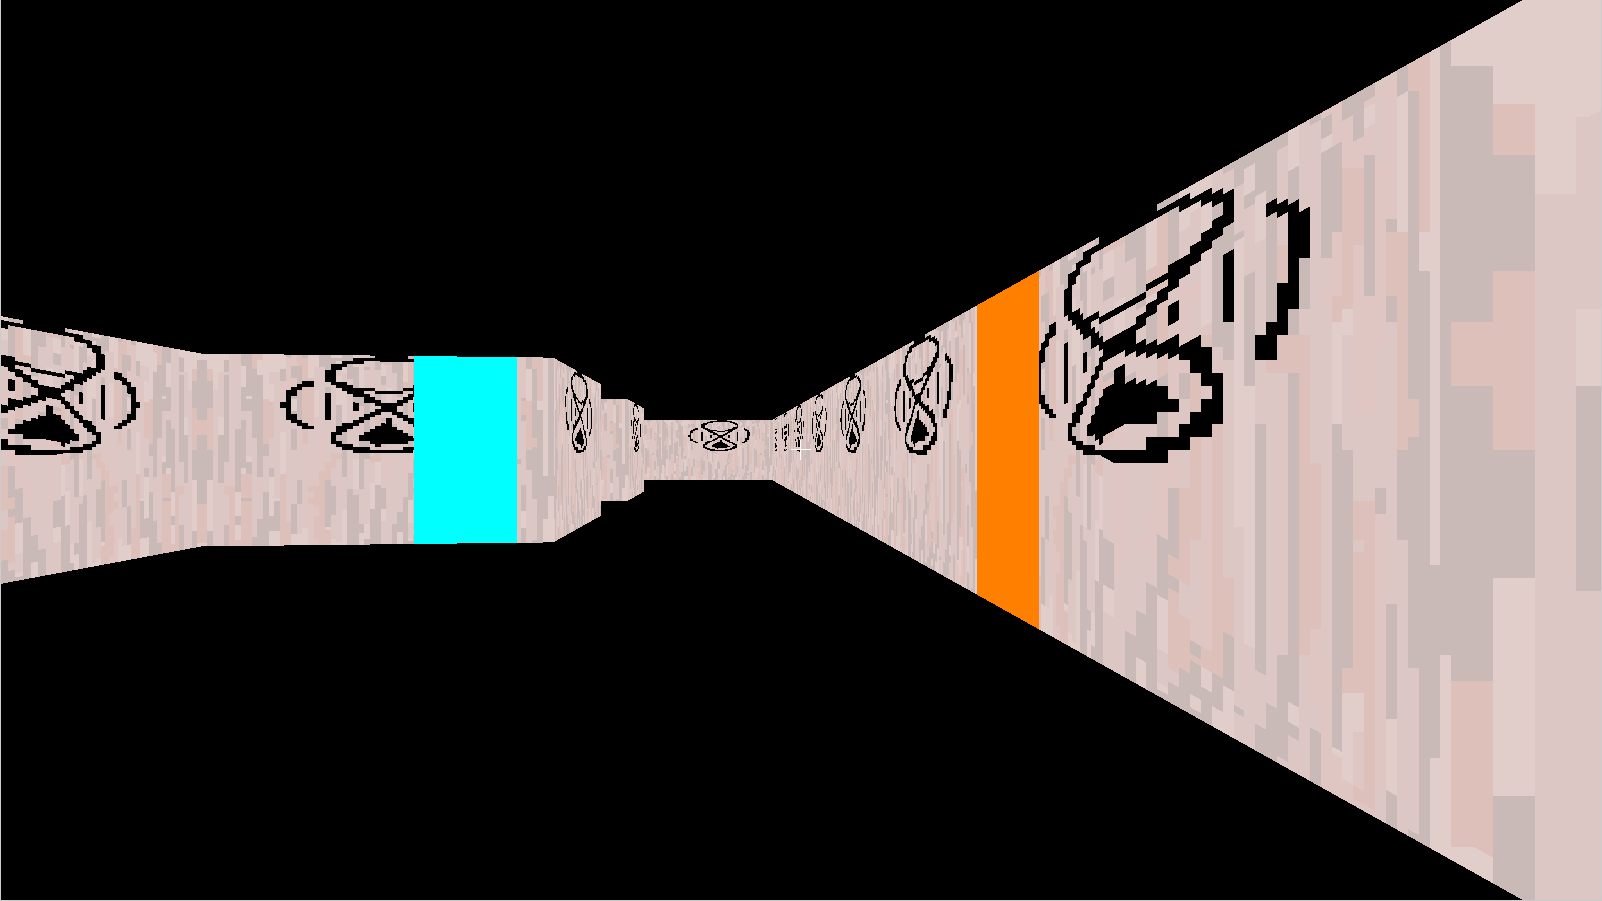
\includegraphics[width=1\textwidth]{image/Portal0.0.png}

	\vfill % Insertion d'un espace vertical flexible pour pousser le texte en bas

    \begin{minipage}{0.3\textwidth}
        \centering
        
\includegraphics[width=1\textwidth]{image/logo-UFR-ST.jpg} 
    \end{minipage}
	\hfill
    \begin{minipage}{0.4\textwidth}
        \begin{flushright}
            \small Tuteur : Julien BERNARD
        \end{flushright}    
    \end{minipage}

\end{titlepage}



\newpage

\section*{Remerciements}

Nous tenons à remercier notre enseignant de projet, M. \textsc{Bernard} 
qui a volontier accepter notre idée et a su nous conseiller tout au long de ce projet.



\newpage

\tableofcontents

\newpage

\section{Introduction}

Portal 0.0 est un jeu vidéo de type puzzle à la première personne.
Il est une version très simplifiée du jeu \href{https://fr.wikipedia.org/wiki/Portal_(jeu_vid%C3%A9o)}{Portal}\cite{Portal}
qui utilise un moteur de type Raycaster à la façon du jeu
\href{https://fr.wikipedia.org/wiki/Wolfenstein_3D}{Wolfenstein 3D}\cite{Wolfenstein3D} pour afficher les éléments
du jeu.

Lors de ce rapport, nous allons détailler les différents aspects conceptuels et
techniques de ce projet. 
Nous commencerons par présenter les besoins et les objectifs du projet. 
Ensuite, nous détaillerons les algorithmes et les technologies utilisés et mis en place pour mettre en oeuvre ce projet.
Comme la creation des murs, les collisions et les différentes stratégies envisagées pour le rendu 3D.
Suivit des explication sur des parties importantes des implantations de ces algorithmes.
Enfin nous pourrons conclure sur ce projet en détaillant ce qui a finalement été réalisé par rapport à ce qui était prévu
ainsi que les perspectives d'avenir pour ce projet.

\section{Besoins et objectifs du projet}
\subsection{Contexte}

\begin{figure}
	\begin{minipage}{0.48\textwidth}
		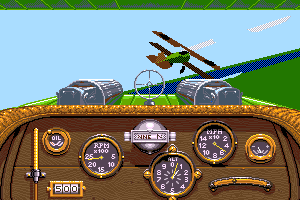
\includegraphics[width=\linewidth]{image/knights-of-the-sky.png}
		\hspace*{-0.5cm}
		\caption{Knights of the Sky}
		\label{fig:knights-of-the-sky}
	\end{minipage}
	\begin{minipage}{0.48\textwidth}
		\centering
		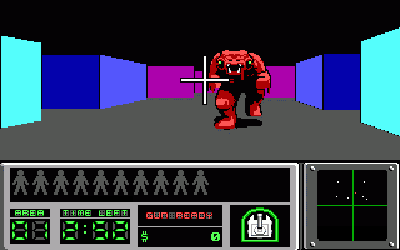
\includegraphics[width=\linewidth]{image/Hovertank_3D.png}
		\hspace*{-0.5cm}
		\caption{Hovertank 3D}
		\label{fig:hovertank3d}
	\end{minipage}
\end{figure}

\begin{figure}
	\begin{minipage}{0.48\textwidth}
		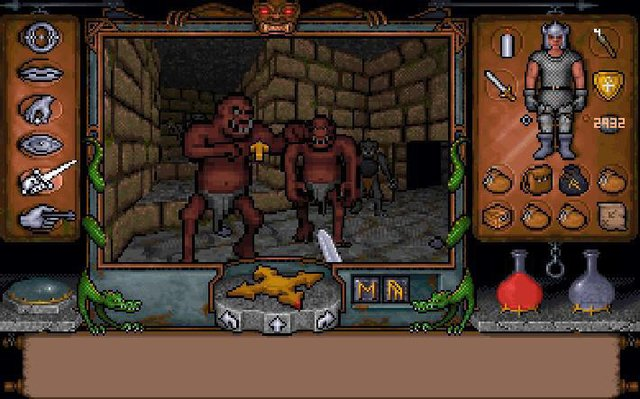
\includegraphics[width=\linewidth]{image/Ultima_Underworld.jpg}
		\hspace*{-0.5cm}
		\caption{Ultima Underworld}
		\label{fig:ultimaunderworld}
	\end{minipage}
	\begin{minipage}{0.48\textwidth}
		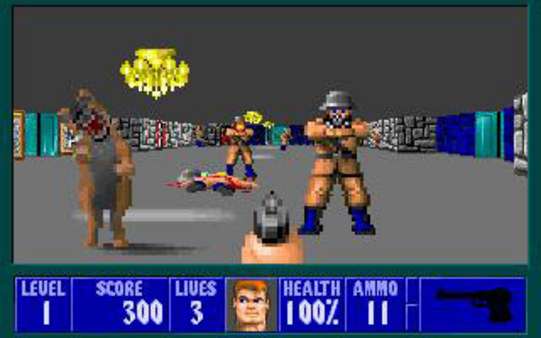
\includegraphics[width=\linewidth]{image/wolfenstein_3d.jpg}
		\hspace*{-0.5cm}
		\caption{Wolfenstein 3D}
		\label{fig:wolfenstein3d}
	\end{minipage}
\end{figure}

\begin{figure}
	\begin{minipage}{0.48\textwidth}
		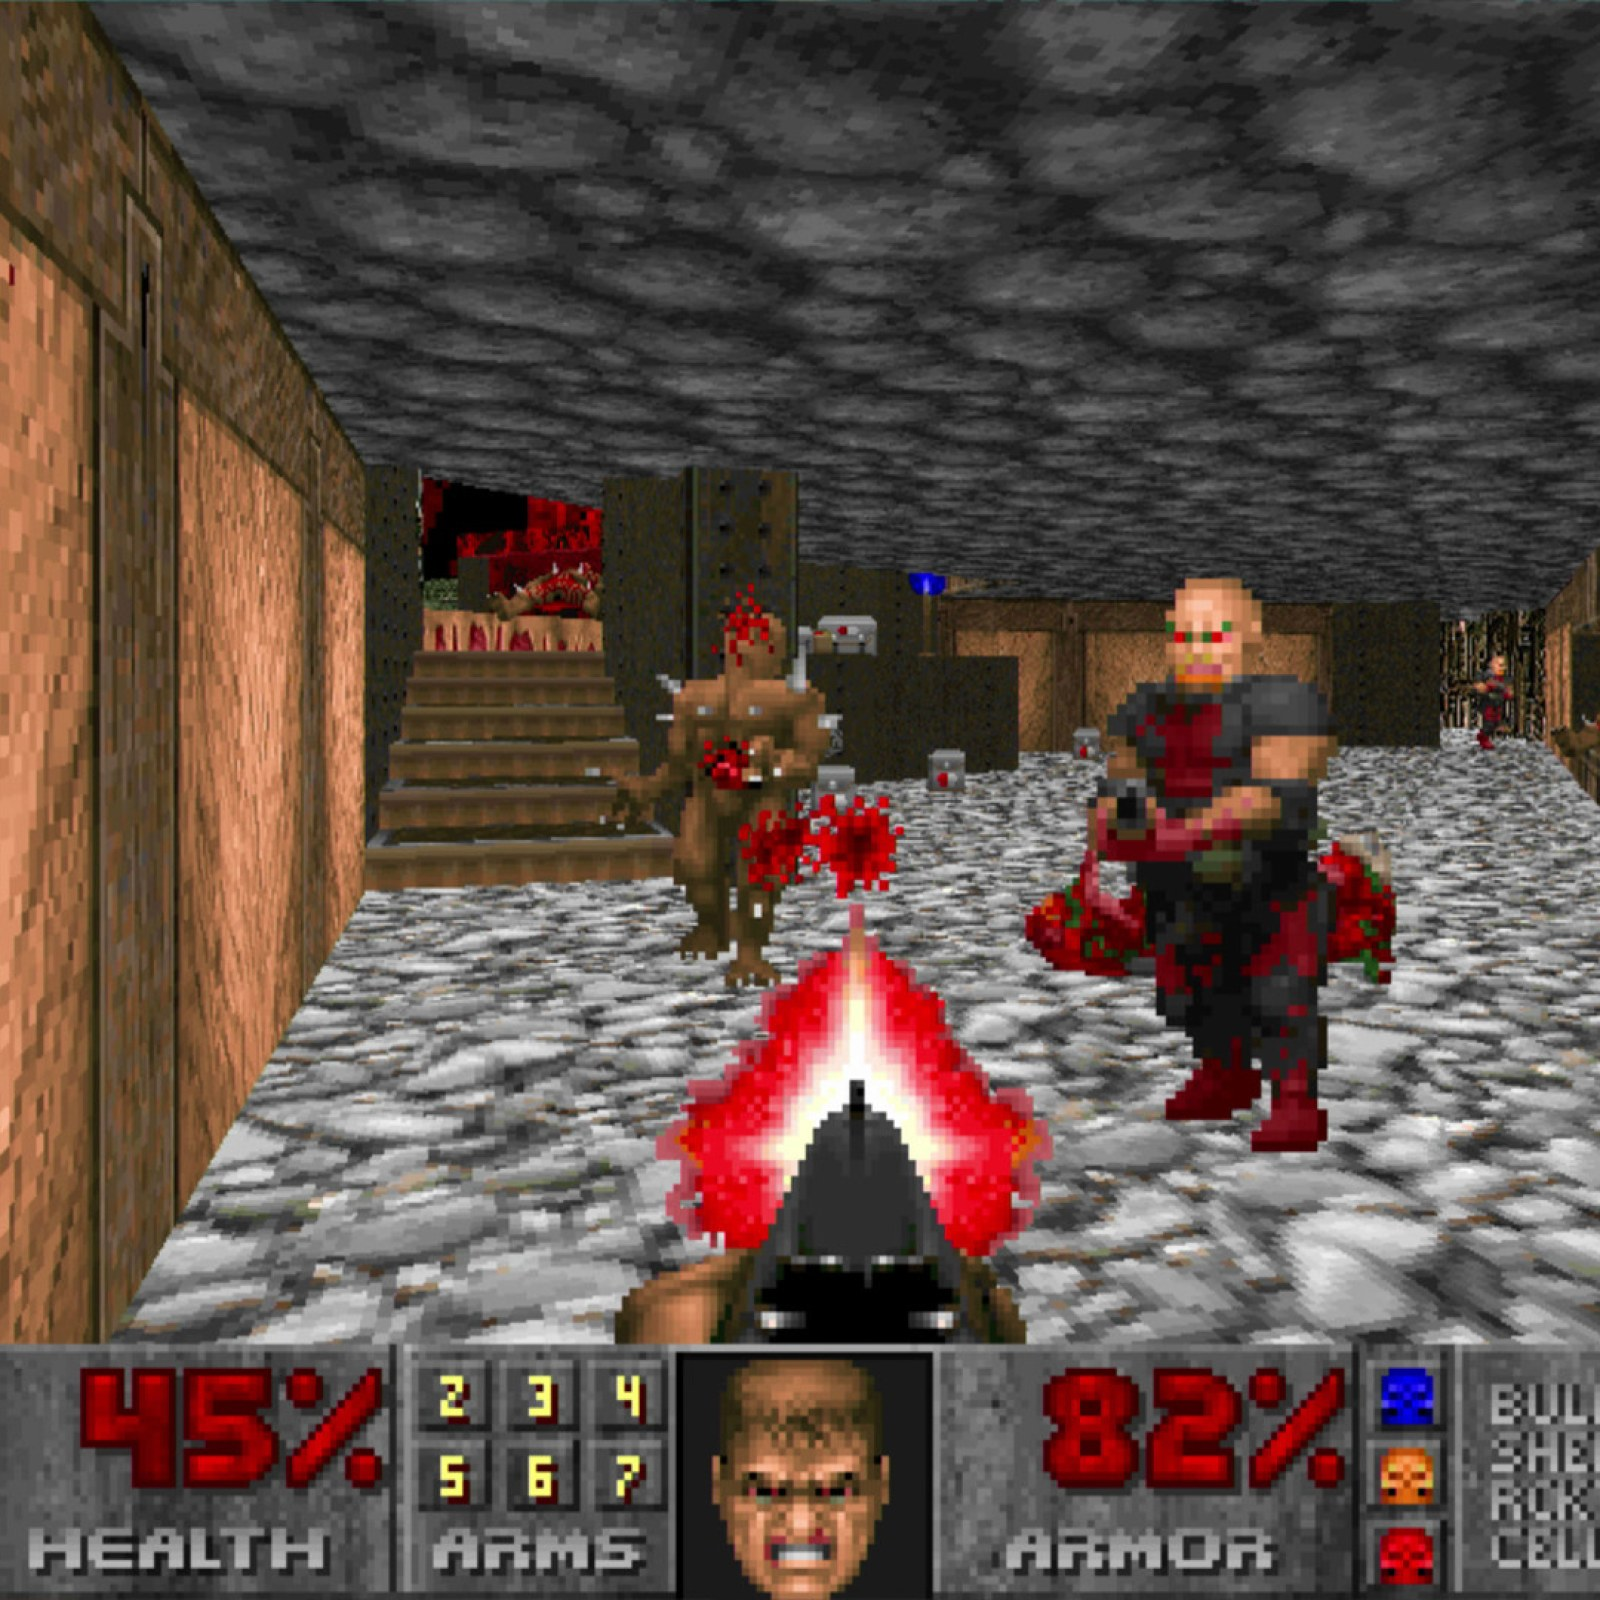
\includegraphics[width=\linewidth]{image/doom_1993.jpg}
		\hspace*{-0.5cm}
		\caption{Doom (1993)}
		\label{fig:doom_1993} 
	\end{minipage}
	\begin{minipage}{0.48\textwidth}
		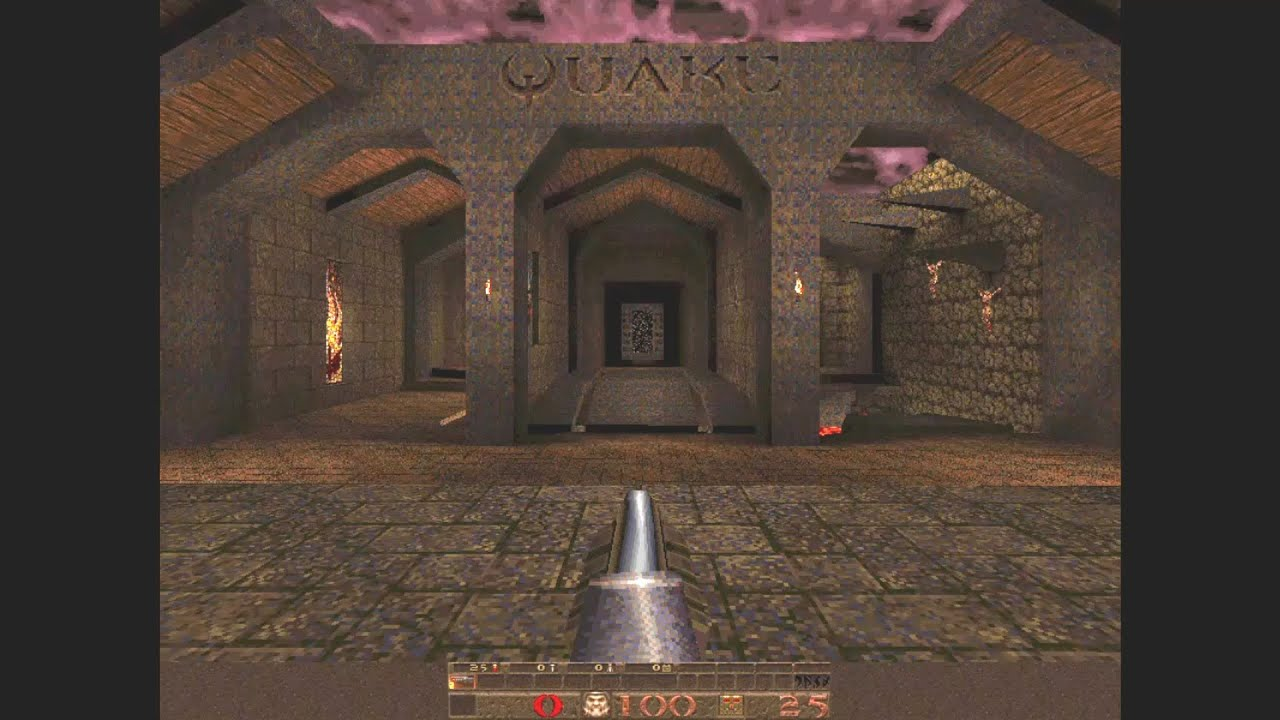
\includegraphics[width=\linewidth]{image/quake_1996.jpg}
		\hspace*{-0.5cm}
		\caption{Quake (1996)}
		\label{fig:quake_1996}
	\end{minipage}
\end{figure}


\paragraph{Les graphismes :}
Au début des années 90, la société \href{https://fr.wikipedia.org/wiki/Id_Software}{Id Software}\cite{Id_Software} a entrepris des 
recherches pionnières dans le domaine des graphismes 3D, alors principalement réservés aux simulateurs de vols tels 
que \href{https://fr.wikipedia.org/wiki/Wing_Commander_(jeu_vid%C3%A9o)}{Wing Commander}\cite{Wing_Commander} ou 
\href{https://en.wikipedia.org/wiki/Knights_of_the_Sky}{Knights of the Sky}\cite{Knights_of_the_Sky} (\nameref{fig:knights-of-the-sky}), deux titres parus en 1990. Face aux 
contraintes de performance des ordinateurs de l'époque, le développement de jeux d'action en 3D rapide représentait 
un défi de taille. C'est dans ce contexte que \href{https://fr.wikipedia.org/wiki/John_Carmack}{John Carmack}\cite{John_Carmack} a 
proposé l'utilisation de la technique du \href{https://fr.wikipedia.org/wiki/Raycasting}{raycasting}\cite{Raycasting}, permettant 
de calculer uniquement les surfaces visibles par le joueur. En six semaines, Carmack développe un moteur 3D innovant 
utilisant des sprites 2D pour représenter les entités du jeu. Ce moteur a été utilisé dans le jeu 
\href{https://fr.wikipedia.org/wiki/Hovertank_3D}{Hovertank 3D}\cite{Hovertank3D} (\nameref{fig:hovertank3d}), publié en avril 1991.
À l'automne 1991, alors que \href{https://fr.wikipedia.org/wiki/John_Carmack}{John Carmack}\cite{John_Carmack} et 
\href{https://fr.wikipedia.org/wiki/John_Romero}{John Romero}\cite{John_Romero} finalisaient le moteur de 
\href{https://en.wikipedia.org/wiki/Commander_Keen_in_Goodbye,_Galaxy}{Commander Keen in Goodbye, Galaxy}\cite{Commander_Keen_in_Goodbye_Galaxy}, Carmack 
découvre \href{https://fr.wikipedia.org/wiki/Ultima_Underworld}{Ultima Underworld}\cite{Ultima_Underworld} (\nameref{fig:ultimaunderworld}), un jeu développé par 
\href{https://fr.wikipedia.org/wiki/Looking_Glass_Studios}{Blue Sky Productions}\cite{Looking_Glass_Studios} (qui deviendra plus tard Looking Glass Studios), 
doté d'un moteur capable de rendre des graphismes 3D texturés sans subir les limitations de Hovertank 3D.
Inspiré, Carmack décide d'améliorer son propre moteur pour 
intégrer le mapping de textures tout en conservant de hautes performances. Après un intense travail de six semaines, 
le nouveau moteur 3D est achevé et utilisé pour le jeu \href{https://fr.wikipedia.org/wiki/Catacomb_3D}{Catacomb 3D}\cite{Catacomb3D},
publié en novembre 1991. La révélation de Catacomb 3D a poussé 
\href{https://fr.wikipedia.org/wiki/Scott_Miller_(programmeur)}{Scott Miller}\cite{Scott_Miller} d'Apogee à convaincre l'équipe de 
développer un jeu d'action en 3D sous forme de shareware. Cela a conduit au lancement du projet 
\href{https://fr.wikipedia.org/wiki/Wolfenstein_3D}{Wolfenstein 3D}\cite{Wolfenstein3D} (\nameref{fig:wolfenstein3d}), un remake en 3D de 
\href{https://fr.wikipedia.org/wiki/Castle_Wolfenstein}{Castle Wolfenstein}\cite{Castle_Wolfenstein}. Sorti le 5 mai 1992 sur PC, ce jeu a 
non seulement été un succès commercial mais a également posé les bases du genre du jeu de tir à la première personne, 
préfigurant ainsi des titres légendaires tels que 
\href{https://fr.wikipedia.org/wiki/Doom_(jeu_vid%C3%A9o,_1993)}{Doom}\cite{Doom_1993} (\nameref{fig:doom_1993}) et 
\href{https://fr.wikipedia.org/wiki/Quake}{Quake}\cite{Quake} (\nameref{fig:quake_1996}).

\begin{figure}
	\centering
	\href{https://fr.wikipedia.org/wiki/Portal_(jeu_vid%C3%A9o)}{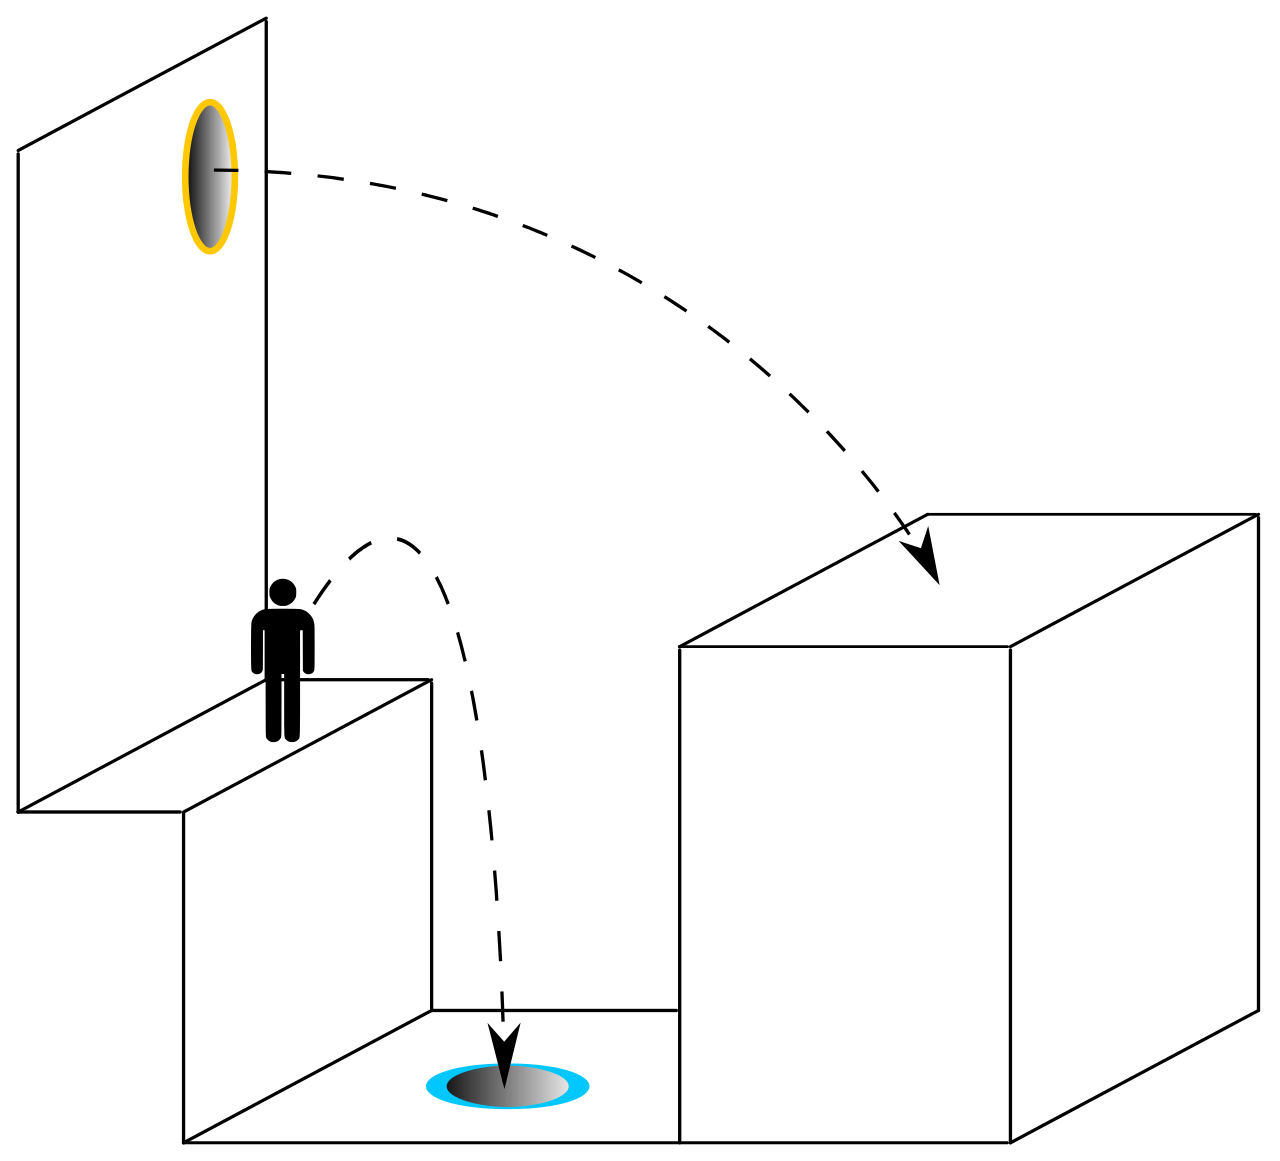
\includegraphics[width=0.5\textwidth]{image/schema_portal.png}}
	\hspace*{-0.5cm}
	\caption{Schéma de fonctionnement du système de portail}
	\label{fig:schema_portal}
\end{figure}

\paragraph{Le système de jeu : }
En 2007, \href{https://fr.wikipedia.org/wiki/Valve_Corporation}{Valve Corporation}\cite{Valve_Corporation} a révolutionné le genre des jeux 
de réflexion à la première personne avec la sortie de 
\href{https://fr.wikipedia.org/wiki/Portal_(jeu_vid%C3%A9o)}{Portal}\cite{Portal}. Ce jeu introduit un mécanisme unique 
permettant au joueur de générer deux portails, l'un orange et l'autre bleu, sur des surfaces planes et 
interconnectées. Ces portails offrent la possibilité de traverser instantanément l'espace d'un point à un autre, 
tout en conservant l'inertie. L'objectif est de résoudre divers puzzles en se servant de cette capacité à manipuler 
l'espace pour atteindre la sortie des différents niveaux proposés.



\subsection{Motivations}


L'une des motivations principales de ce projet est de réaliser un jeu vidéo
avec graphique comme à l'époque de \href{https://fr.wikipedia.org/wiki/Wolfenstein_3D}{Wolfenstein 3D}\cite{Wolfenstein3D}
mais avec des concepts de jeux plus récentes et qui plus pourrait être
un préquel de \href{https://fr.wikipedia.org/wiki/Portal_(jeu_vid%C3%A9o)}{Portal}\cite{Portal}.
\subsection{Objectifs}
Pour débuter ce projet, des objectifs ont été fixés.
Il a été décidé de réaliser un jeu vidéo en C++ avec la bibliothèque GF.
Le moteur de rendu devait être de type Raycaster pour imiter les graphismes
de \href{https://fr.wikipedia.org/wiki/Wolfenstein_3D}{Wolfenstein 3D}\cite{Wolfenstein3D}.
Aussi, comme le nom du jeu l'indique, il était nécessaire d'implanter un système de portail,
par lesquels le joueur pourrait se déplacer d'un point à un autre et voir au travers.

\section{Algorithmes et technologies}
\subsection{Création des murs}
\begin{figure}
	\centering
	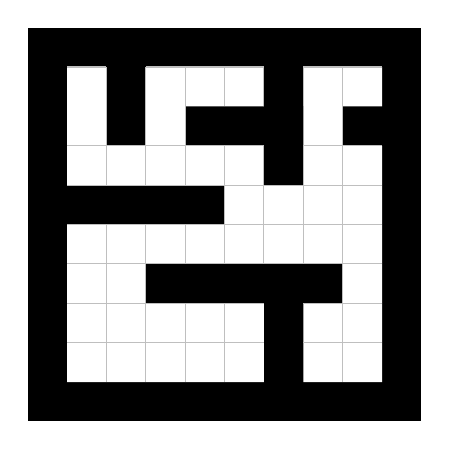
\begin{tikzpicture}[scale=0.5]

		\fill[line width=1pt] (0, 0) -- (0, 10) -- (10, 10) -- (10, 0) -- cycle;
		\fill[white] (1, 1) -- (6, 1) -- (6, 3) -- (3, 3) -- (3, 4) -- (8, 4) -- (8, 3) -- (7, 3) -- (7, 1) -- (9, 1) -- (9, 7) -- (8, 7) -- (8, 8) -- (9, 8) -- (9, 9) -- (7, 9) -- (7, 6) -- (6, 6) -- (6, 7) -- (4, 7) -- (4, 8) -- (6, 8) -- (6, 9) -- (3, 9) -- (3, 7) -- (2, 7) -- (2, 9) -- (1, 9) -- (1, 6) -- (5, 6) -- (5, 5) -- (1, 5) -- cycle;
	
	
		\draw[color=lightgray] (2, 5) -- (2, 1);
		\draw[color=lightgray] (2, 9) -- (2, 6);
	
		\draw[color=lightgray] (3, 5) -- (3, 1);
		\draw[color=lightgray] (3, 9) -- (3, 6);
	
		\draw[color=lightgray] (4, 3) -- (4, 1);
		\draw[color=lightgray] (4, 5) -- (4, 4);
		\draw[color=lightgray] (4, 9) -- (4, 6);
	
		\draw[color=lightgray] (5, 3) -- (5, 1);
		\draw[color=lightgray] (5, 7) -- (5, 4);
		\draw[color=lightgray] (5, 9) -- (5, 8);
	
		\draw[color=lightgray] (6, 7) -- (6, 4);
		\draw[color=lightgray] (6, 9) -- (6, 8);
	
		\draw[color=lightgray] (7, 7) -- (7, 4);
		\draw[color=lightgray] (7, 9) -- (7, 8);
		\draw[color=lightgray] (8, 9) -- (8, 1);
	
	
		\draw[color=lightgray] (1, 9) -- (2, 9);
		\draw[color=lightgray] (3, 9) -- (6, 9);
		\draw[color=lightgray] (7, 9) -- (9, 9);
	
		\draw[color=lightgray] (1, 7) -- (6, 7);
		\draw[color=lightgray] (7, 7) -- (9, 7);
	
		\draw[color=lightgray] (1, 6) -- (9, 6);
	
		\draw[color=lightgray] (1, 5) -- (9, 5);
		
		\draw[color=lightgray] (1, 4) -- (9, 4);
	
		\draw[color=lightgray] (1, 3) -- (6, 3); 
		\draw[color=lightgray] (7, 3) -- (9, 3);
		
		\draw[color=lightgray] (1, 2) -- (6, 2); 
		\draw[color=lightgray] (7, 2) -- (9, 2);
		
	\end{tikzpicture}
	\caption{PNG d'une carte}
	\label{fig:png_map}
\end{figure}

% Dans cette partie nous allons détailler les différentes étapes pour la création des murs.

\subsubsection{Les cartes}
Afin de pouvoir afficher des cartes, nous avons dû créer un fichier PNG\footnote{Portable Network Graphics} où nous dessinons les murs ainsi que la case de départ et d'arrivée (\nameref{fig:png_map}). Lors du lancement du jeu, le programme lit le fichier PNG et enregistre les différentes cases dans un tableau à deux dimensions. En même temps, le programme va regarder si les coordonnées correspondent à une cellule de mur, la case de départ, la case d'arrivée ou aucune des trois. Si c'est une cellule de mur, alors on va effectuer un parcours en profondeur des coordonnées adjacentes pour savoir si ceux sont des cellules de murs ou non. Grâce à cela nous pouvons récuperer toutes les cellules d'un mur directement et ainsi compter le nombre de mur assez facilement.


\subsubsection{Récupération des sommets utiles}
Pour la création des murs, on effectue une boucle sur la liste de coordonnées des cellules occupées par un mur précédemment récupérée. Sur chacune des coordonnées, on regarde quatre de ses coordonnées adjacentes qui représente les cellules en haut, en bas, à gauche et à droite. Si l'une d'entre elles fait partie de la liste des coordonnées des murs alors on incrémente un compteur. Si ce compteur est égal à 1 ou 3 alors on ajoute les coordonnées essayées dans une liste de coordonnées dites utiles, c'est-à-dire que ce sont les coordonnées des sommets des murs.

\subsubsection{Tri des sommets}
Afin de faciliter le rendu des murs, nous avons besoin de trier les sommets. Pour cela, nous effectuons une boucle tant que la taille de la liste des sommets utiles est supérieure à la taille de la liste des sommets triés. Dans cette boucle, nous effectuons une boucle sur la liste des sommets utiles si le sommet est dans la liste des sommets triés ou non. S'il ne l'est pas alors on récupère les coordonnées de ce sommet et fait appel à une fonction pour trier à partir de ce sommet, la liste des sommets utiles et la liste des sommets triés. Dans cette fonction, on effectue une boucle sur la liste des sommets utiles à partir du sommet donné en paramètre. On regarde pour chaque sommet s'il existe un sommet dans la direction choisie ainsi que dans sa direction opposée. %(Explication de la fonction fctCanGo?)
\begin{itemize}
	\item S'il existe un sommet dans la direction choisie et aucun sommet dans la direction opposée alors on ajoute ce sommet dans la liste des sommets triés.
	\item Sinon s'il existe un sommet dans la direction opposée et aucun sommet dans la direction choisie alors on ajoute le sommet de la direction opposée dans la liste des sommets triés et changer la direction courante par la direction opposée.
	\item Sinon
	\begin{itemize}
		\item S'il existe un sommet dans la direction choisie et un sommet dans la direction opposée alors on regarde si le sommet de la direction opposée n'est pas dans la liste des sommets triés et qu'un changement de direction doit être effectué ou bien que le sommet de la direction choisie est dans la liste des sommets triés et qu'un changement de direction ne doit pas être effectué alors on va ajouter le sommet de la direction opposée dans la liste des sommets triés et changer la direction courante par la direction opposée.
		\item Sinon on ajoute le sommet de la direction choisie dans la liste des sommets triés.
	\end{itemize}
\end{itemize}

On change de direction en fonction de la direction courante, si le changement de direction reste le même que l'ancien alors on va changer de direction. Si n'existe aucun sommet dans les directions choisies et opposées alors on va incrémenter un compteur. Si ce compteur est supérieur ou égal à 4 alors on arrête la fonction de tri.

\subsubsection{Contruction des murs}
Une fois les sommets utiles triés nous allons pouvoir construire les murs et les ajouter dans une liste de murs. Chaque mur de cette liste a pour attributs les coordonnées de ses sommets triés, les coordonnées de ses cellules occupées et la taille de son périmètre.

\subsection{Les collisions}

Dans ce point nous allons traiter des collisions. Notre objectif est d'empêcher
que notre personnage puisse se déplacer à travers les murs.

\subsubsection{Aspect conceptuel}

\begin{figure}
	\centering
	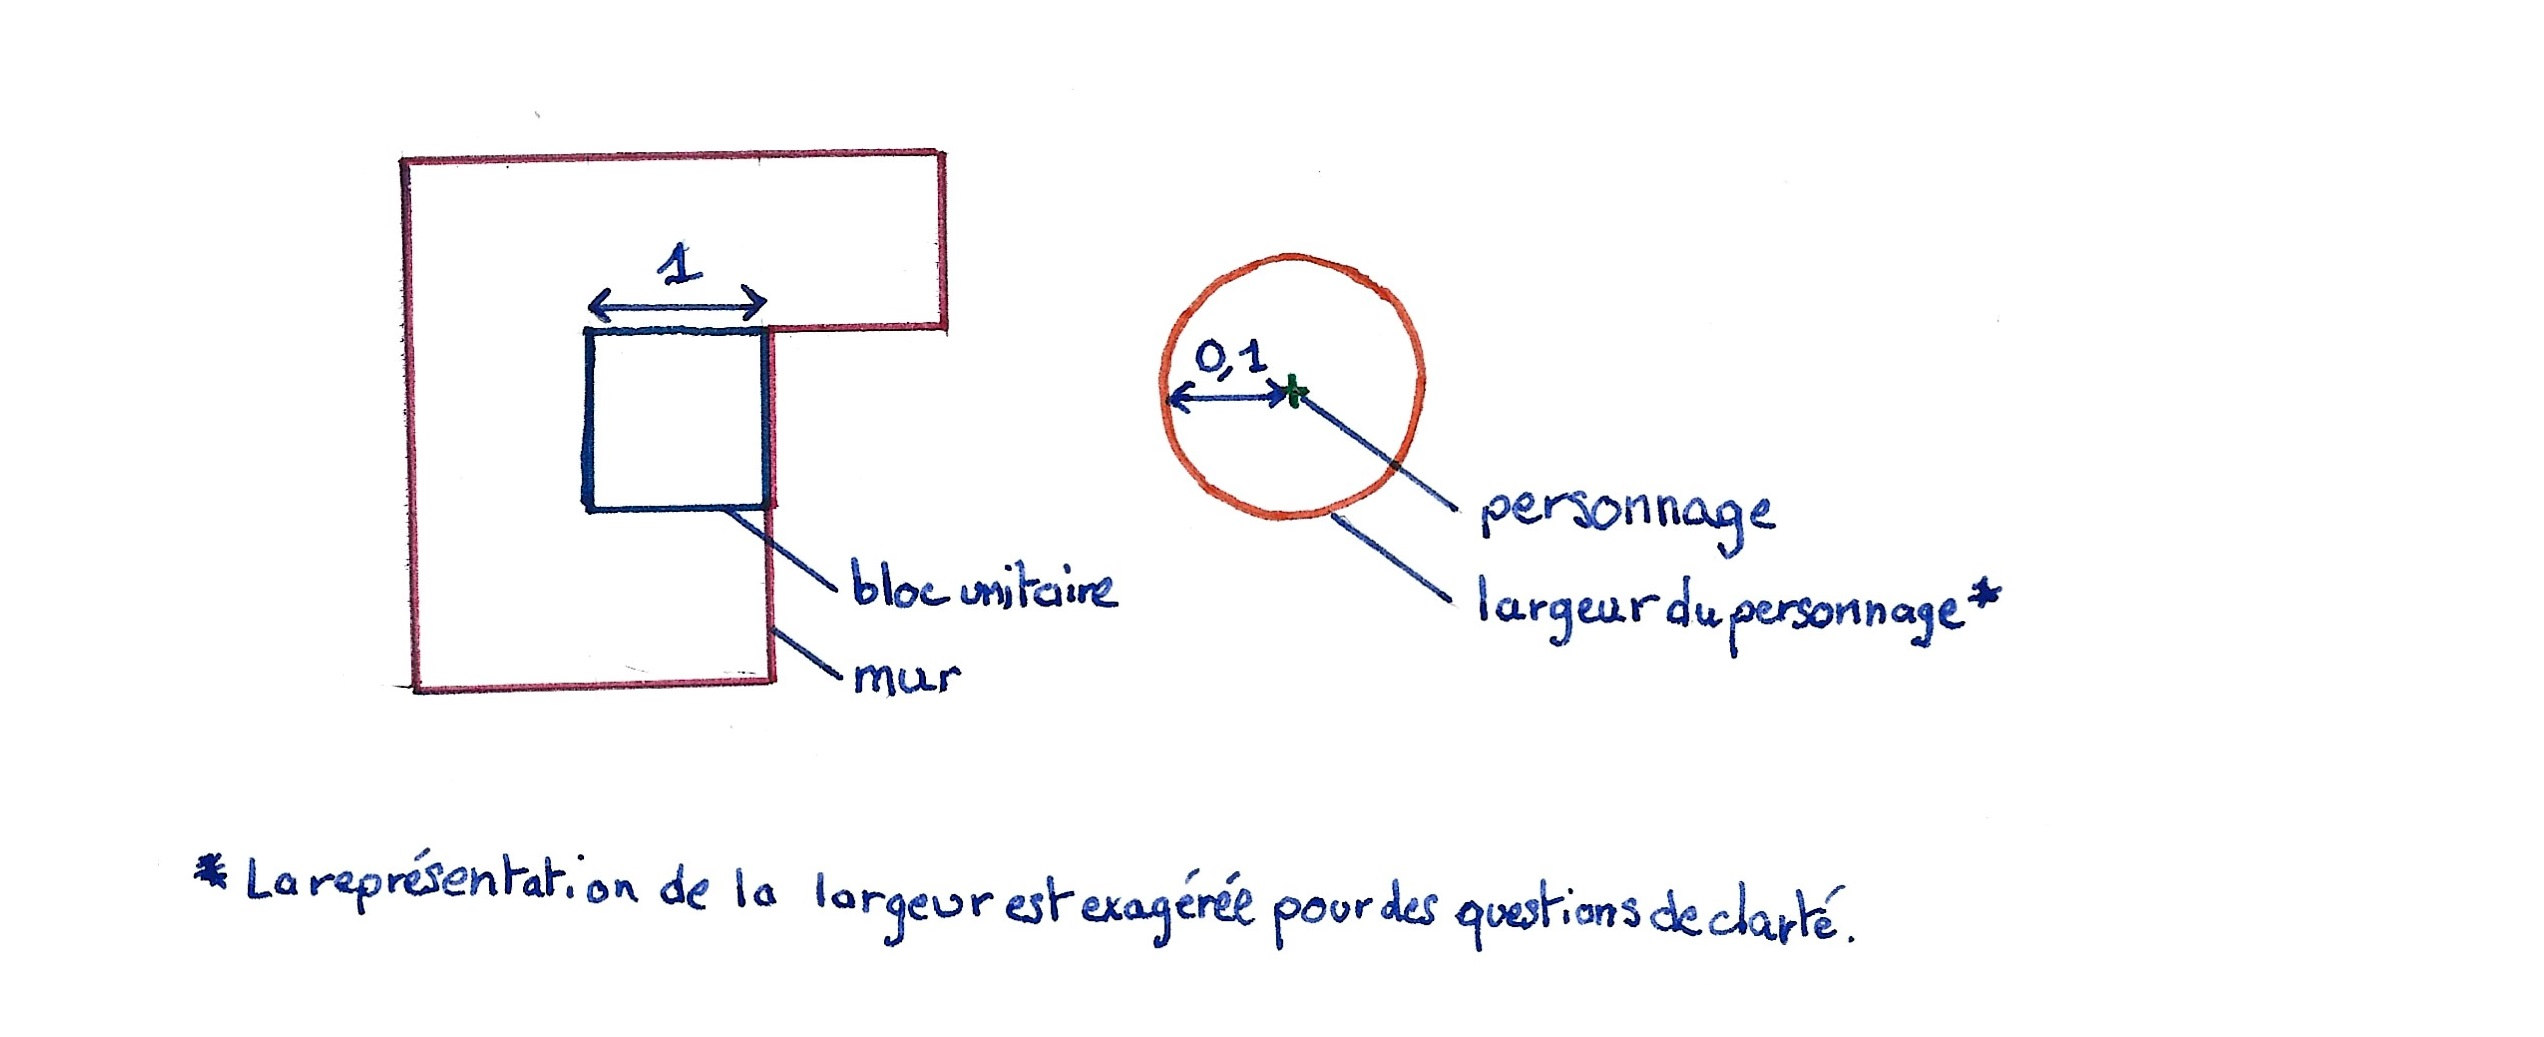
\includegraphics[width=1\textwidth]{image/fig1.jpg}
	\caption{Collision cercle/rectangle}
	\label{fig:collision_cercle_rectangle}
\end{figure}

% Nous commençons avec l'aspect conceptuel.
Le personnage est représenté par un point auquel nous accordons une largeur et donc un cercle centré autour de lui.
Chaque mur est composé de blocs carrés unitaires.
Ainsi, nous employons un système de collision entre un cercle et un rectangle (cf: \nameref{fig:collision_cercle_rectangle}). 

Ce système s'appuie sur une méthode de "clampage", qui permet de connaître le point du mur le plus proche.
Puis, à l'aide de la distance entre ce point et le personnage, on détermine si notre cercle est en collision avec notre rectangle.

Alors deux cas se présentent à nous:

\begin{figure}
	\begin{minipage}{0.48\textwidth}
		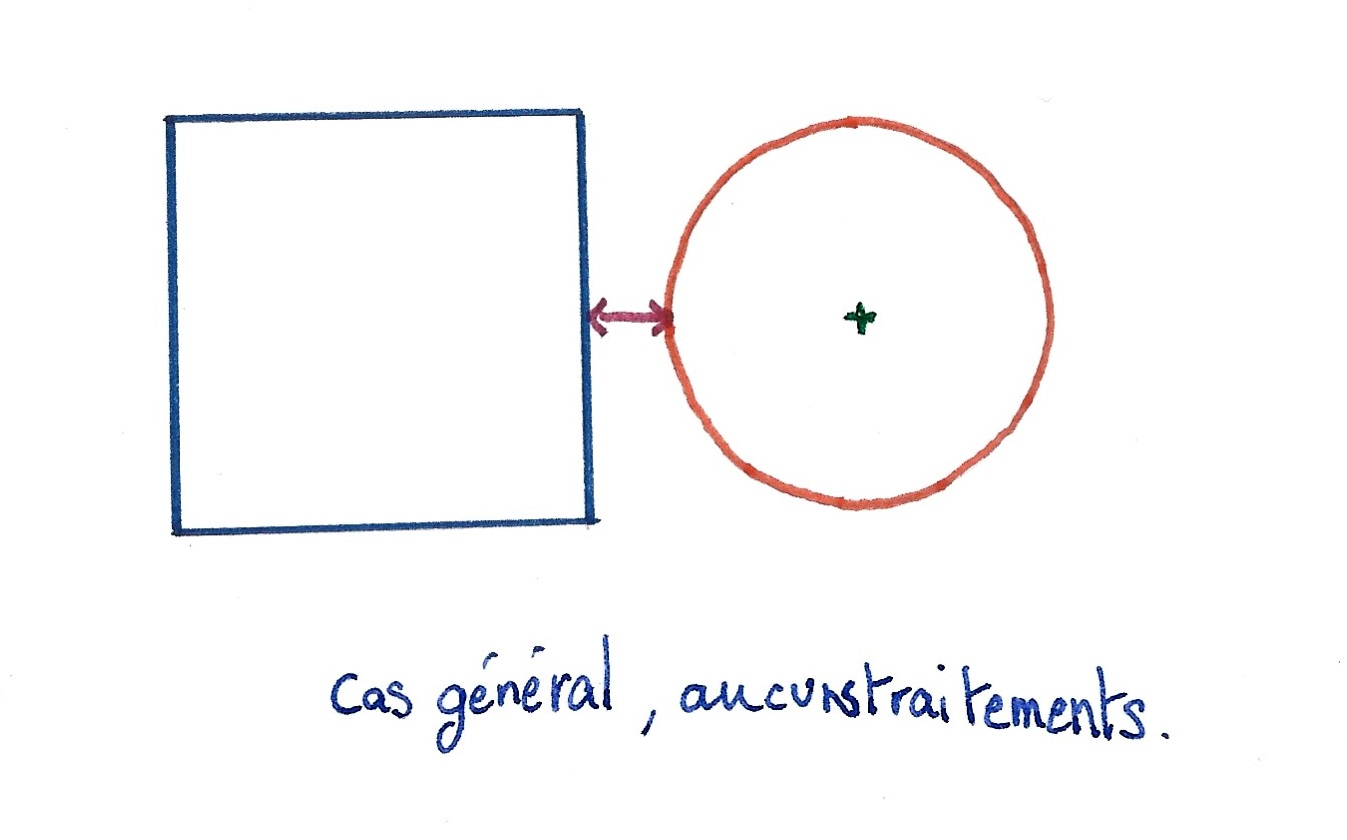
\includegraphics[width=\linewidth]{image/fig2.jpg}
		\caption{Pas de collision}
		\label{fig:pas_de_collision}
	\end{minipage}
	\begin{minipage}{0.48\textwidth}
		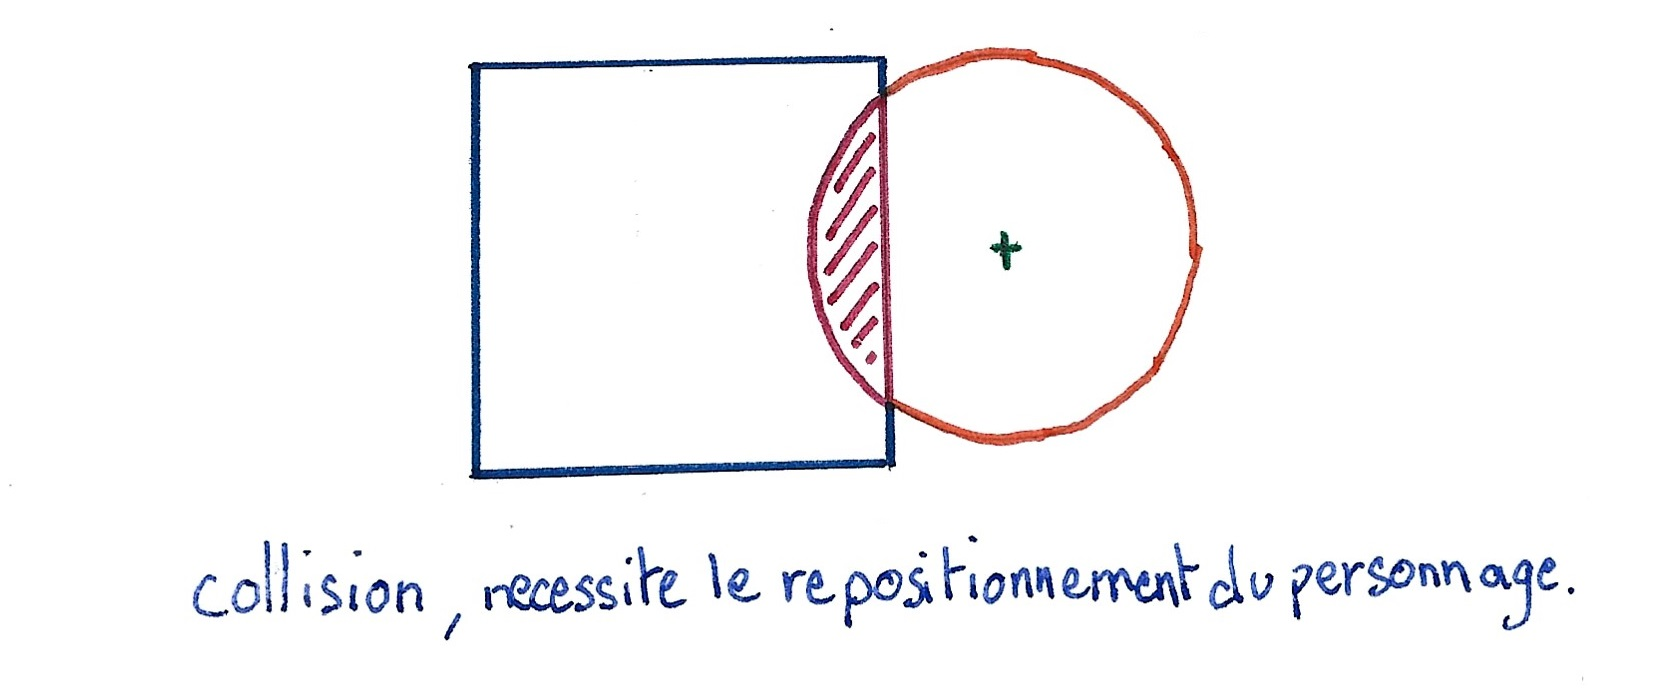
\includegraphics[width=\linewidth]{image/fig3.jpg}
		\caption{Collision}
		\label{fig:collision}
	\end{minipage}
\end{figure}

\paragraph{Premier cas :} 

Le cercle n'est pas en collision avec le rectangle, alors aucun traitement spécifique n'est à prévoir (cf: \nameref{fig:pas_de_collision}). 

\paragraph{Second cas :} 

Le cercle est en collision avec le rectangle (cf: \nameref{fig:collision}) et nous repositionnons le personnage de manière à ce qu'il ne soit plus imbriqué avec le rectangle. 
Ce qui donne un effet visuel de glissement contre le rectangle.

\subsubsection{Aspect technique}

Nous définissons notre personnage, noté P, par des coordonnées représentant sa position ainsi qu'un nombre représentant sa largeur, noté $l$ Ainsi :

$$\text{P} = ((x ; y) ; l), x, y, l \in \mathbb{R}$$ 
$$l = 0.1$$

La méthode de "clampage" consiste à prendre la valeur la plus proche d'une valeur donnée dans un intervalle donnée.
Ce qui nous donne l'applica\-tion suivante :

\begin{align*}
    \text{clamp}\colon\mathbb{R}&\longrightarrow \mathopen{[}a\,;b\mathclose{]}, a\,, b \in \mathbb{R}\\
    x&\longmapsto  \left \{ \begin{array}{c} a \text{ si } x \leq a \\ b \text{ si } x \geq b \\ x \text{ sinon} \end{array} \right.
\end{align*}

A partir de cette application, nous pouvons trouver le point le plus proche 
d'un mur. Nos murs sont composés de blocs unitaires, c'est-à-dire que ce 
sont des carrées de longueur de côté 1. Pour expliquer le procéder, nous 
prenons un de ces blocs, que l'on notera B, et qui est représenté par 
l'ensemble des coordonnées des ses sommets. Pour se repérer dans l'espace, 
il suffit d'une coordonnée pour avoir toutes les autres. Nous choisissons 
arbitrairement de prendre la coordonnée à la plus basse abscisse et plus 
basse ordonnée du bloc que nous noterons (a ; b). Nous avons alors :


$$\text{B} = \{(a ; b) ; (a + 1 ; b) ; (a ; b + 1) ; (a + 1 ; b + 1)\}$$

Que l'on simplifie par

$$\text{B} = (a ; b)$$

\begin{figure}
	\centering
	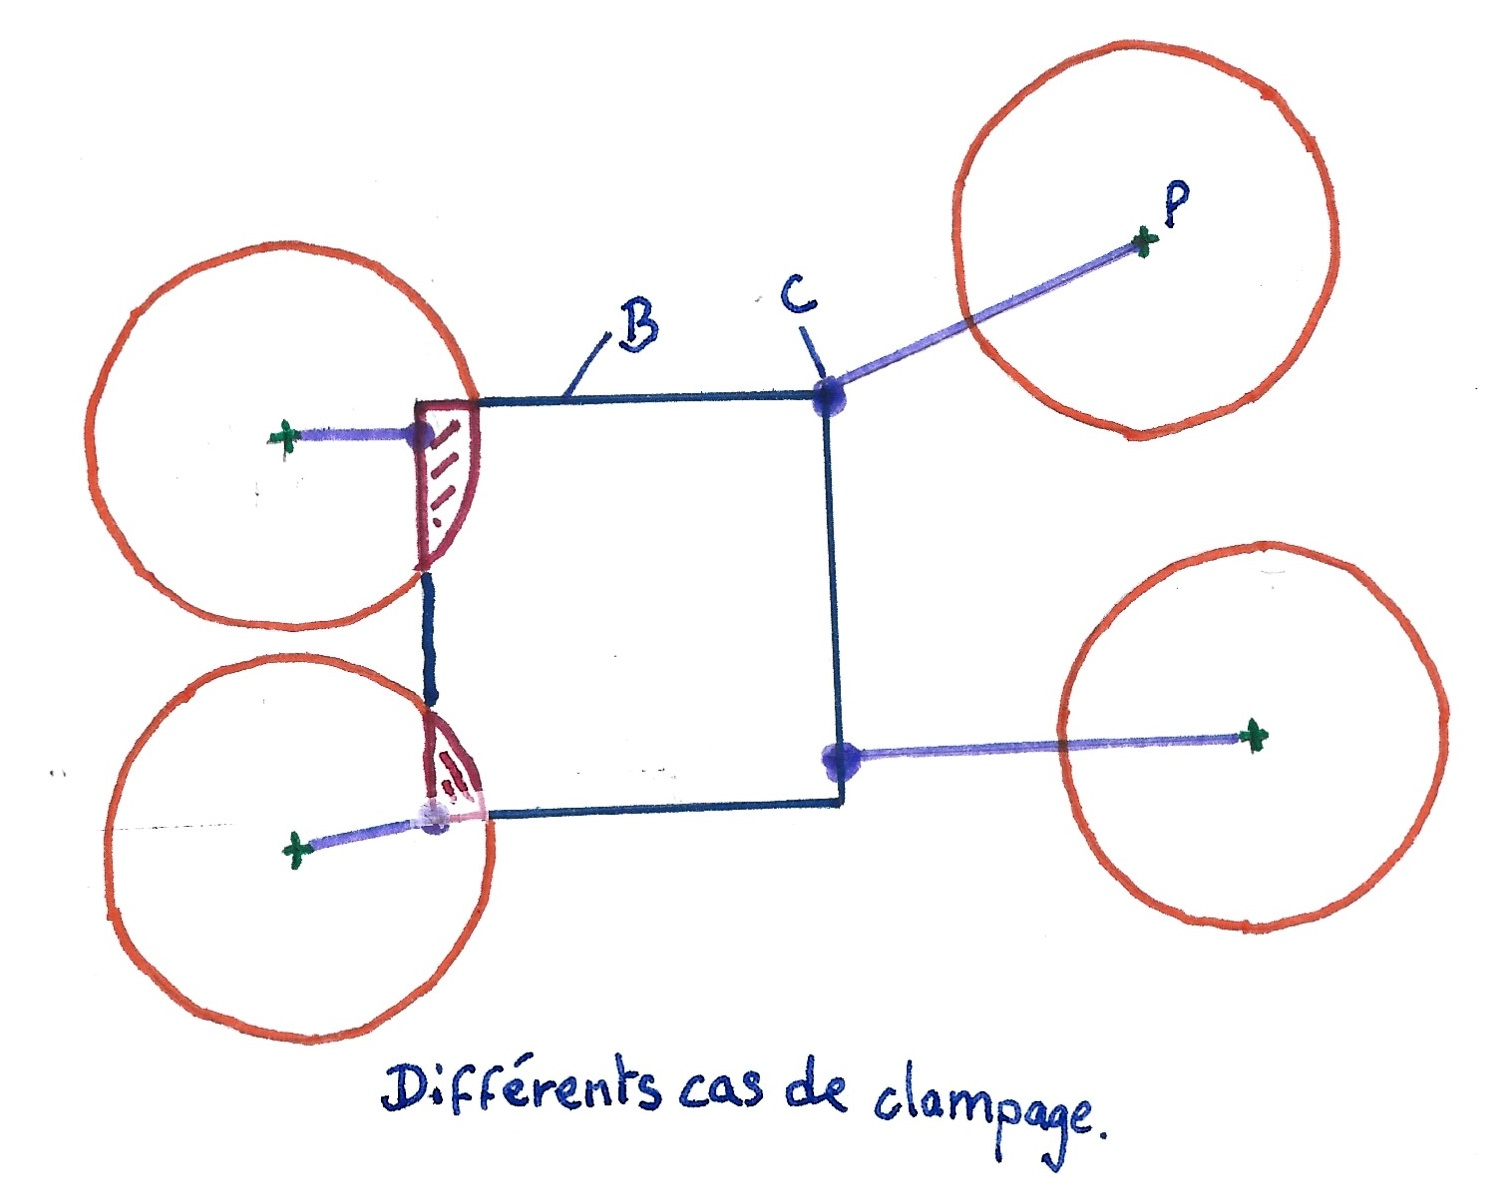
\includegraphics[width=0.5\textwidth]{image/fig4.jpg}
	\caption{Clampage}
	\label{fig:clampage}
\end{figure}

Pour avoir le point le plus proche de B, noté C, nous devons alors "clamper" 
l'abscisse (resp. l'ordonnée) du personnage sur l'intervalle d'abscisse 
(resp. d'ordonnée) de B (cf: \nameref{fig:clampage}). Alors :

$$\text{C} = (\text{clamp}(\text{P}.x, \text{B}.a, \text{B}.a +1) ; \text{clamp}(\text{P}.y, \text{B}.b, \text{B}.b +1))$$

Grâce à C, nous pouvons maintenant vérifier si P est à moins de 0,1 de B, 
et donc en collision. Pour cela, calculons la distance entre P et C :

$$\text{dist} = \sqrt[]{((\text{P}.x - \text{C}.x)^2 + (\text{P}.y - \text{C}.y)^2)}$$

Maintenant, nous pouvons généraliser notre réflexion à un mur pour nous 
offrir une légère optimisation. Nos murs sont composés de plusieurs blocs. 
En appliquant le traitement précédent à chaque bloc et en gardant la 
distance minimale, nous pouvons déterminer le point le plus proche de 
chaque mur cette fois ci. Ceci nous évite des comparaisons inutile par la 
suite. On peut alors définir DistMur :

$$\text{DistMur} = \min(\text{dist})$$

Ensuite, si $\text{distMur} > \text{P}.l$, c'est-à-dire si $\text{dist} > 0,1$, alors P n'entre pas en collision avec B (cf: \nameref{fig:pas_de_collision}). Sinon, nous devons replacer P.

Dans ce second cas, nous devons connaître la nouvelle position de P. Il 
suffit alors d'ajouter la différence entre les coordonnées de P et de C :

$$\text{P} = (\text{P}.x + (\text{P}.x - \text{C}.x) ; \text{P}.y + (\text{P}.y - \text{C}.y))$$

Nous avons donc efficacement mis en place un système de gestion de 
collisions entre un cercle et un rectangle.

\subsection{Différentes stratégies pour le rendu 3D}
Pour implémenter notre jeu, l'un des points les plus importants était de pouvoir afficher des murs en 3D. Pour cela, nous partions d'une grille de cellules 
représentant les emplacements des murs donc d'un environnement 2D pour aller vers un rendu 3D.

\subsubsection{L'algorithme Digital Differential Analyzer (DDA)}

\begin{figure}
	\begin{minipage}{\textwidth}
		\center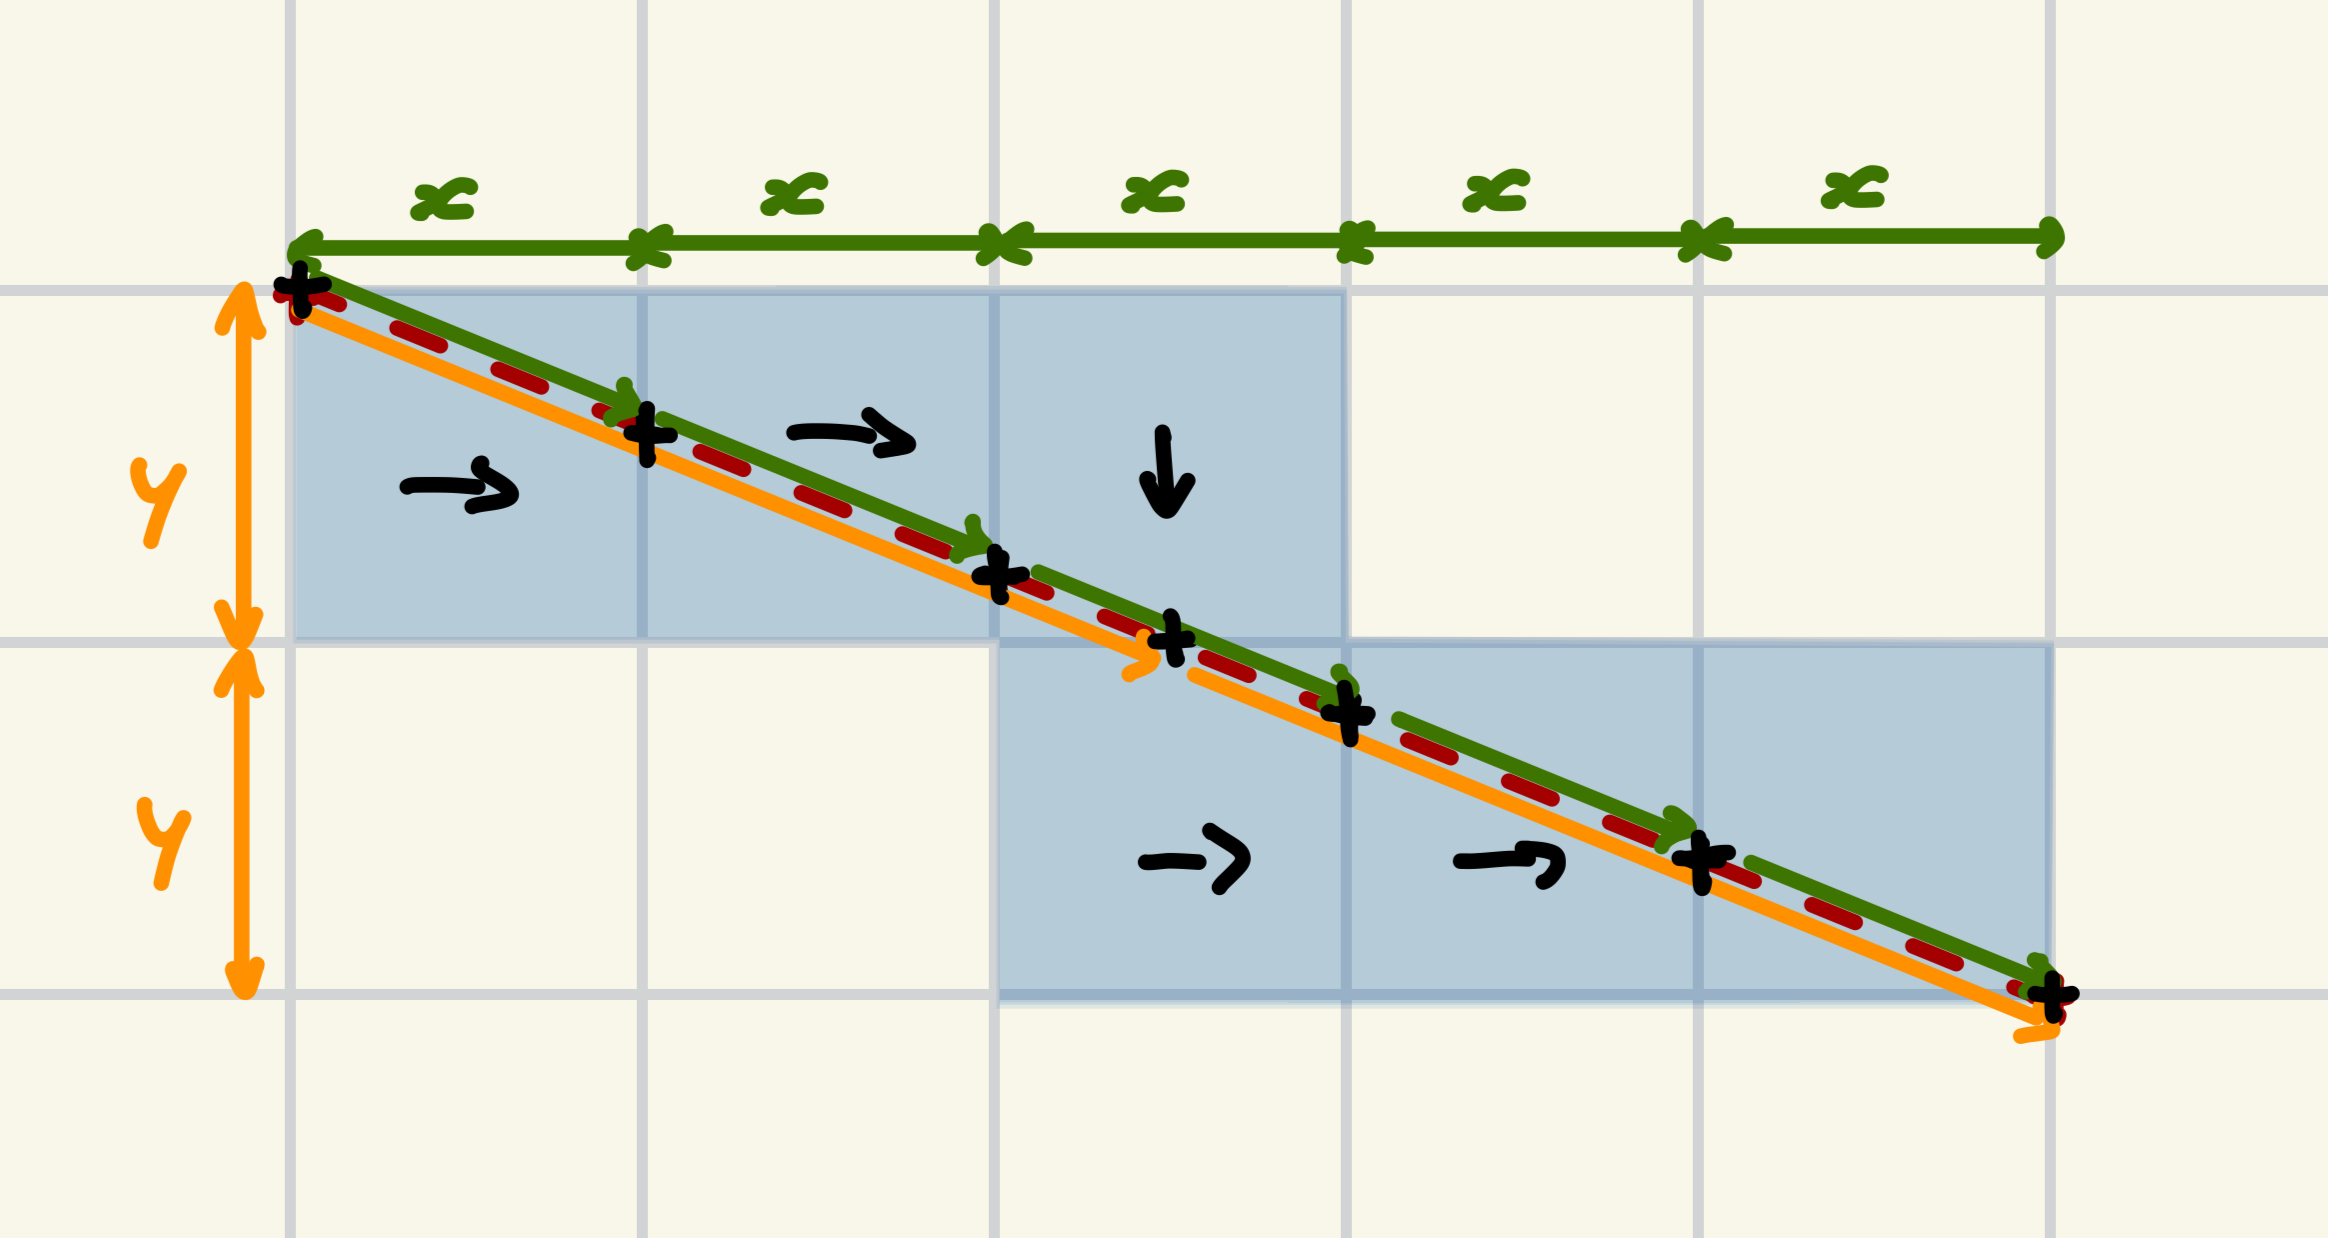
\includegraphics[width=0.8\linewidth]{image/dda1.jpeg}
		\hspace*{-0.5cm}
		\caption{fonctionnement DDA}
		\label{fig:dda1}
	\end{minipage}
\end{figure}

L'algorithme DDA est historiquement conçu pour la rasterisation de lignes, c'est-à-dire la conversion de lignes géométriques en lignes visuelles composées de pixels 
alignés. Dans le contexte du raycasting, DDA est employé pour déterminer où les rayons projetés à travers la scène intersectent avec les objets de l'environnement, 
dans notre cas représenté par une grille de cellules.

Plutôt que de calculer chaque point le long d'une demie droite en utilisant des formules de géométrie 
directe, ce qui pourrait être coûteux en termes de performances, DDA avance par petits incréments. Pour chaque pas sur l'axe le plus 
dominant (x ou y), DDA calcule l'emplacement correspondant sur l'autre axe en ajoutant un incrément constant (cf: \nameref{fig:dda1}). Cela se traduit par un parcours régulier et 
efficace le long de la ligne en faisant des sauts à chaque intersection entre la demie droite et la grille 2D.

Dans le raycasting, DDA est utilisé pour trouver rapidement et précisément les intersections entre les rayons et les murs. 

\subsubsection{Raycasting, l'approche historique}

\begin{figure}
	\center
	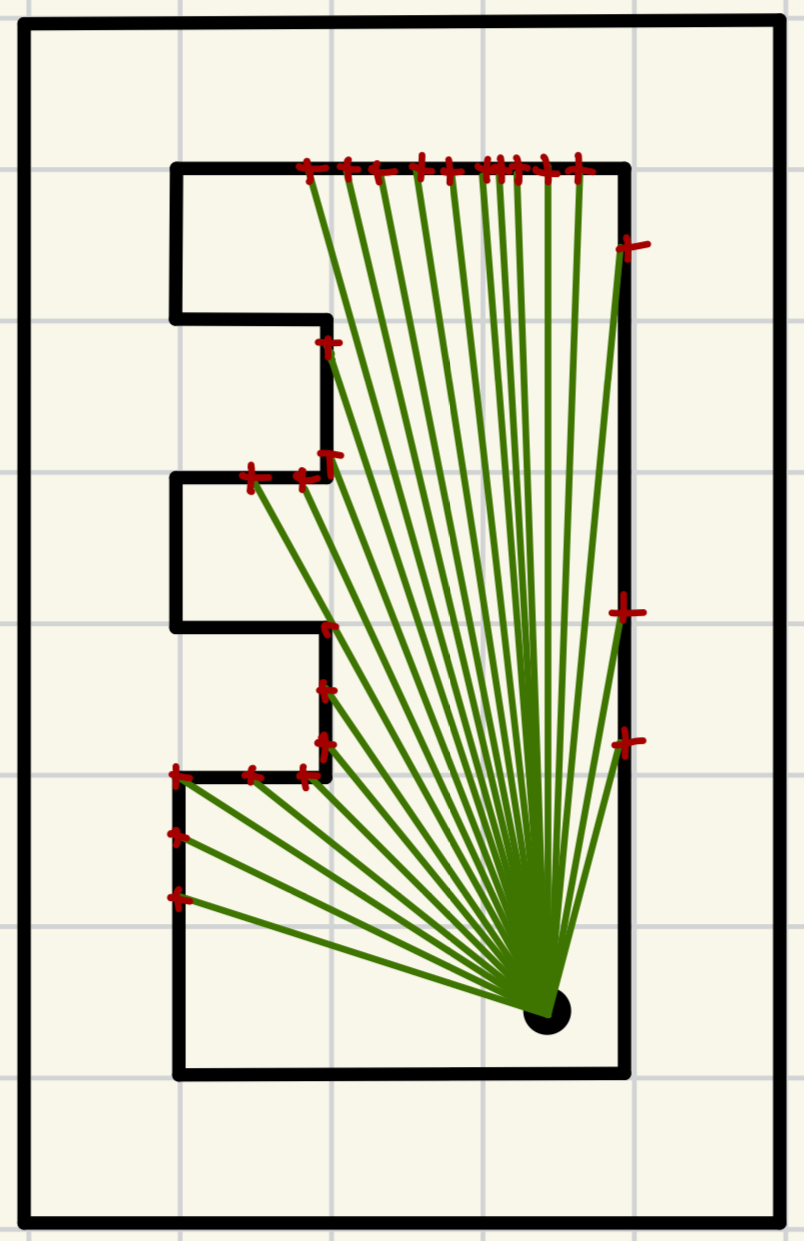
\includegraphics[width=0.25\textwidth]{image/projection2D.jpeg}
	\raisebox{2cm}{
		\hspace{2mm}$\Longrightarrow$\hspace{2mm}
	}
	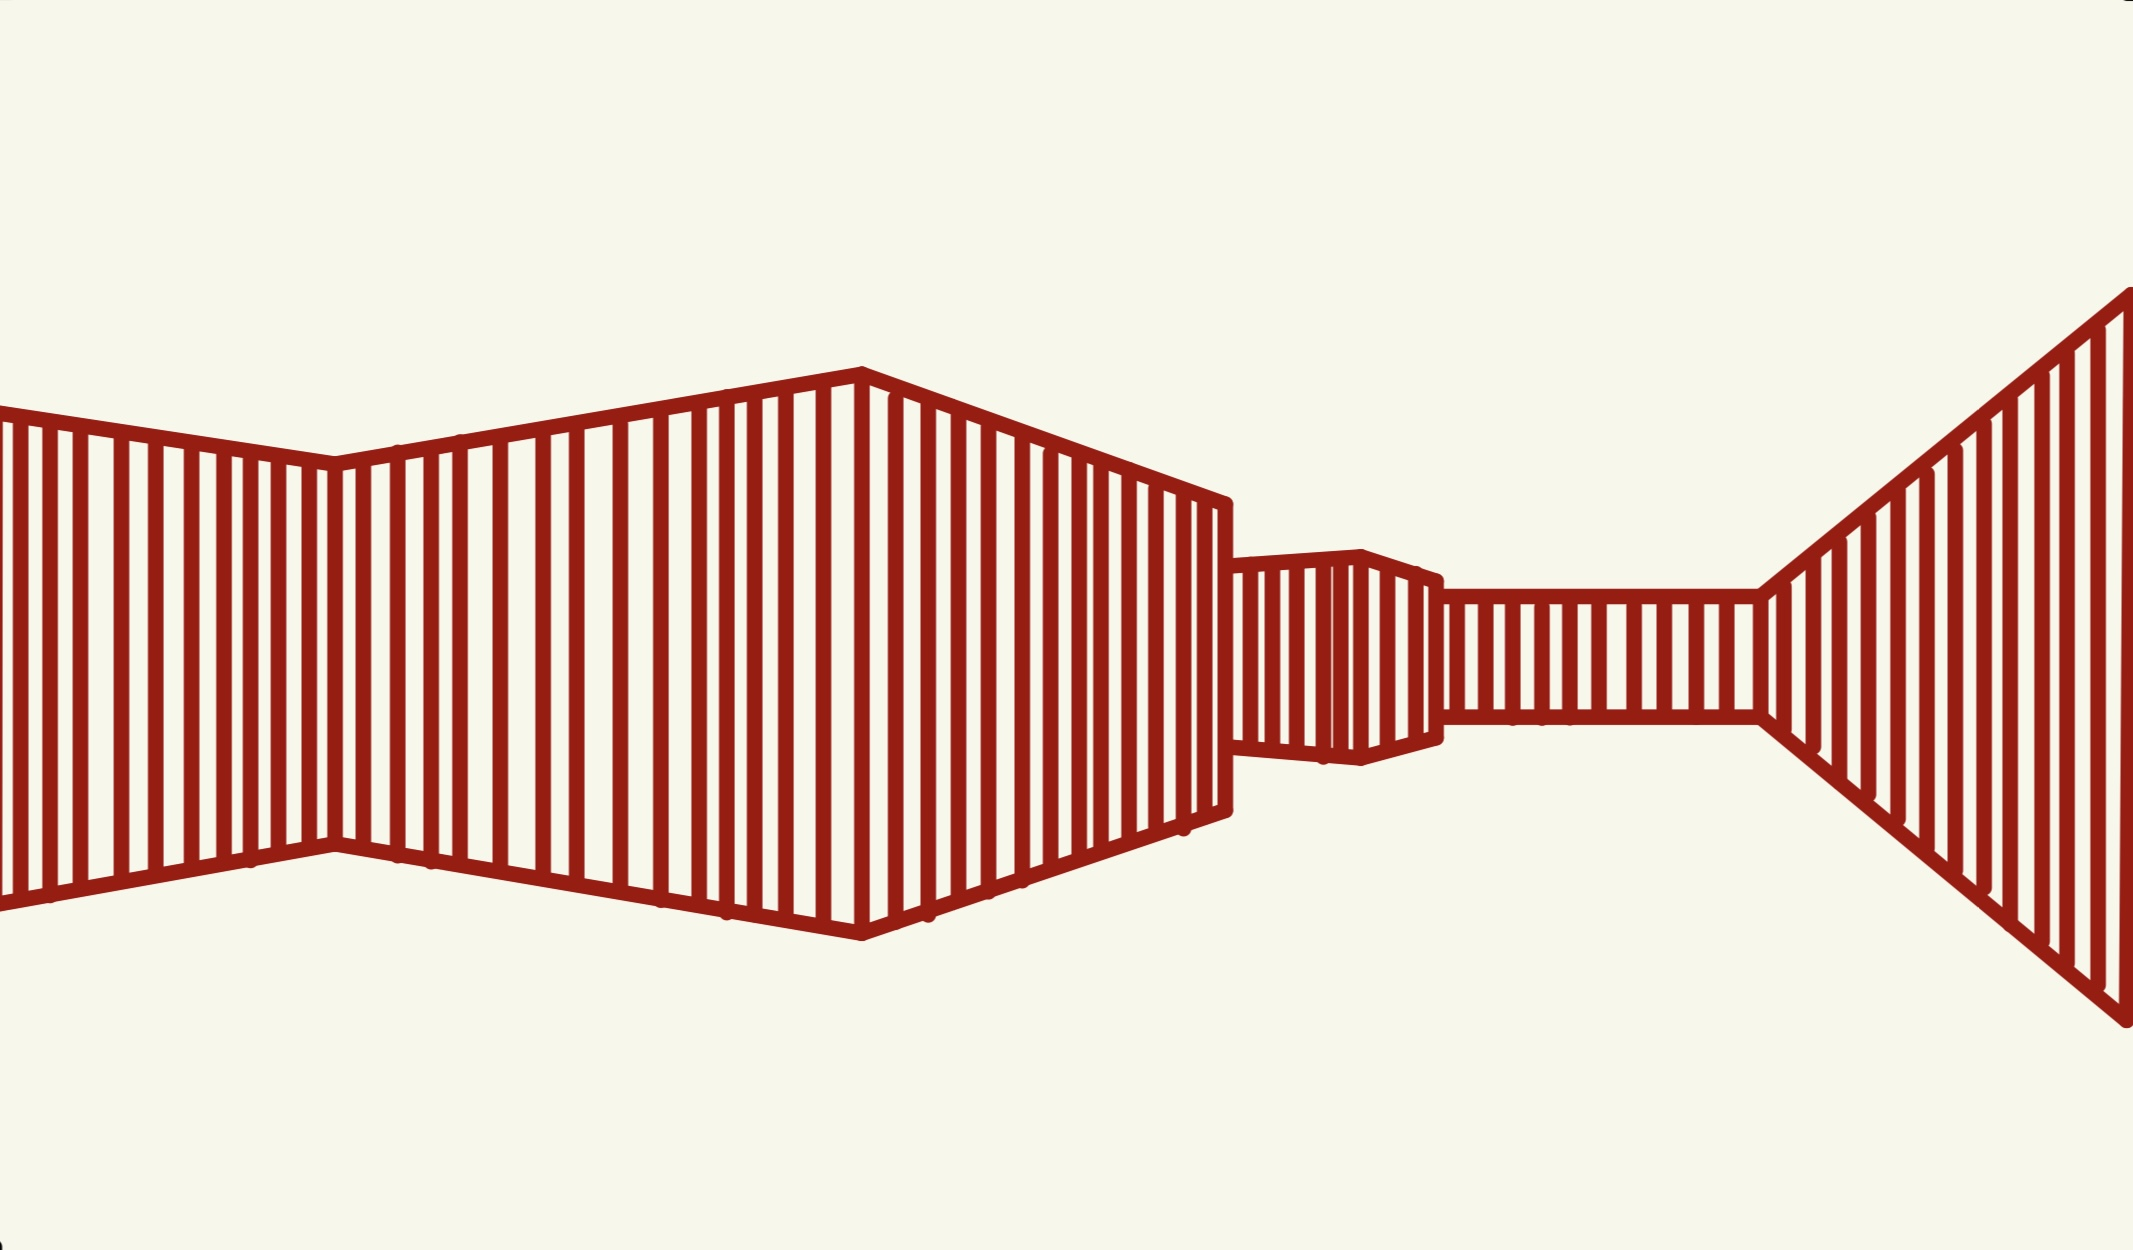
\includegraphics[width=0.6\textwidth]{image/rendu-historique.jpg}
	\caption{résultat historique attendu}
	\label{fig:result-histo}
\end{figure}

La première approche envisagée était celle du raycasting historique.

Historiquement, le raycasting est une méthode de rendu graphique utilisée pour créer une perspective 3D à partir d'un environnement 2D. Cet effet est réalisé en projetant des 
rayons depuis la position du joueur à travers la scène pour déterminer les intersections avec les murs. Pour optimiser ce
processus, l'algorithme (DDA) a été utilisé.

Le raycasting génère une illusion de profondeur en projetant des rayons depuis le point de vue du joueur jusqu'à ce qu'ils rencontrent un 
objet dans l'espace de jeu. Le processus est répété pour chaque colonne de l'écran, permettant ainsi de dessiner une image 3D à partir d'une
carte 2D. Les distances calculées entre le joueur et les points d'intersection sont utilisées pour déterminer la hauteur des objets rendus, 
créant ainsi une perspective en fausse 3D (cf: \nameref{fig:result-histo}).

\paragraph{Les avantages de DDA dans ce contexte :}
\begin{itemize}
\item \textbf{Efficacité :} DDA réduit la quantité de calculs nécessaires pour trouver les intersections. En progressant par 
incréments réguliers, l'algorithme évite les calculs répétés ou complexes typiques des méthodes géométriques standards.
\item \textbf{Précision :} Bien que simple, DDA maintient une précision élevée dans le calcul des intersections. Chaque étape 
avance de manière incrémentielle, garantissant que le rayon suit précisément sa trajectoire prévue sans sauter de pixels ou de cellules.
\item \textbf{Adaptabilité :} L'algorithme s'adapte bien aux grilles de toutes tailles, ce qui le rend idéal pour les jeux avec 
différentes résolutions et des espaces de jeu variés.
\item \textbf{Simplicité et Robustesse :} DDA est relativement simple à implémenter et à comprendre, ce qui réduit le risque 
d'erreurs. Sa robustesse en fait une méthode fiable pour le raycasting dans des environnements de jeu variés.
\end{itemize}

Dans l'application concrète DDA au raycasting, l'algorithme calcule les pas nécessaires pour que le rayon 
traverse une cellule de la grille, soit en horizontal, soit en vertical. Ces pas sont basés sur la direction du 
rayon et sont ajustés à chaque étape pour correspondre à la grille du jeu. Cela permet au rayon de "marcher" à travers 
la grille, cellule par cellule, en vérifiant à chaque pas si un mur a été rencontré.

\noindent Cette approche est assez simple à implémenter, promettant par ailleurs des performances élevées et 
une implémentation de la vue à travers les portails plus aisée. Cependant, cette simplicité est peut être ce qui 
nous a fait choisir une autre approche, plus adaptée à un projet d'étudiants en 3ème année de licence informatique et plus moderne.
 
\subsubsection{Line Of Sight, l'approche moderne}

\begin{figure}
	\center
	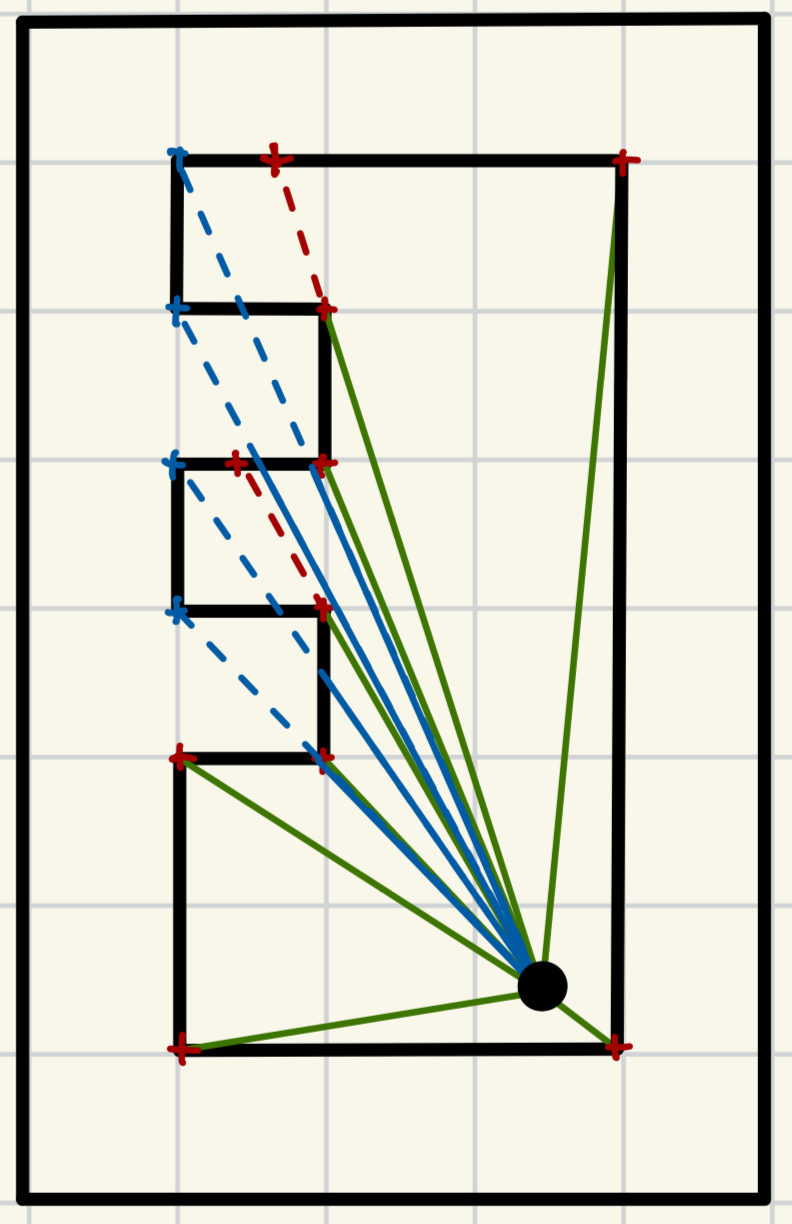
\includegraphics[width=0.25\textwidth]{image/projection-2D-V2.jpeg}
	\raisebox{2cm}{
		\hspace{2mm}$\Longrightarrow$\hspace{2mm}
	}
	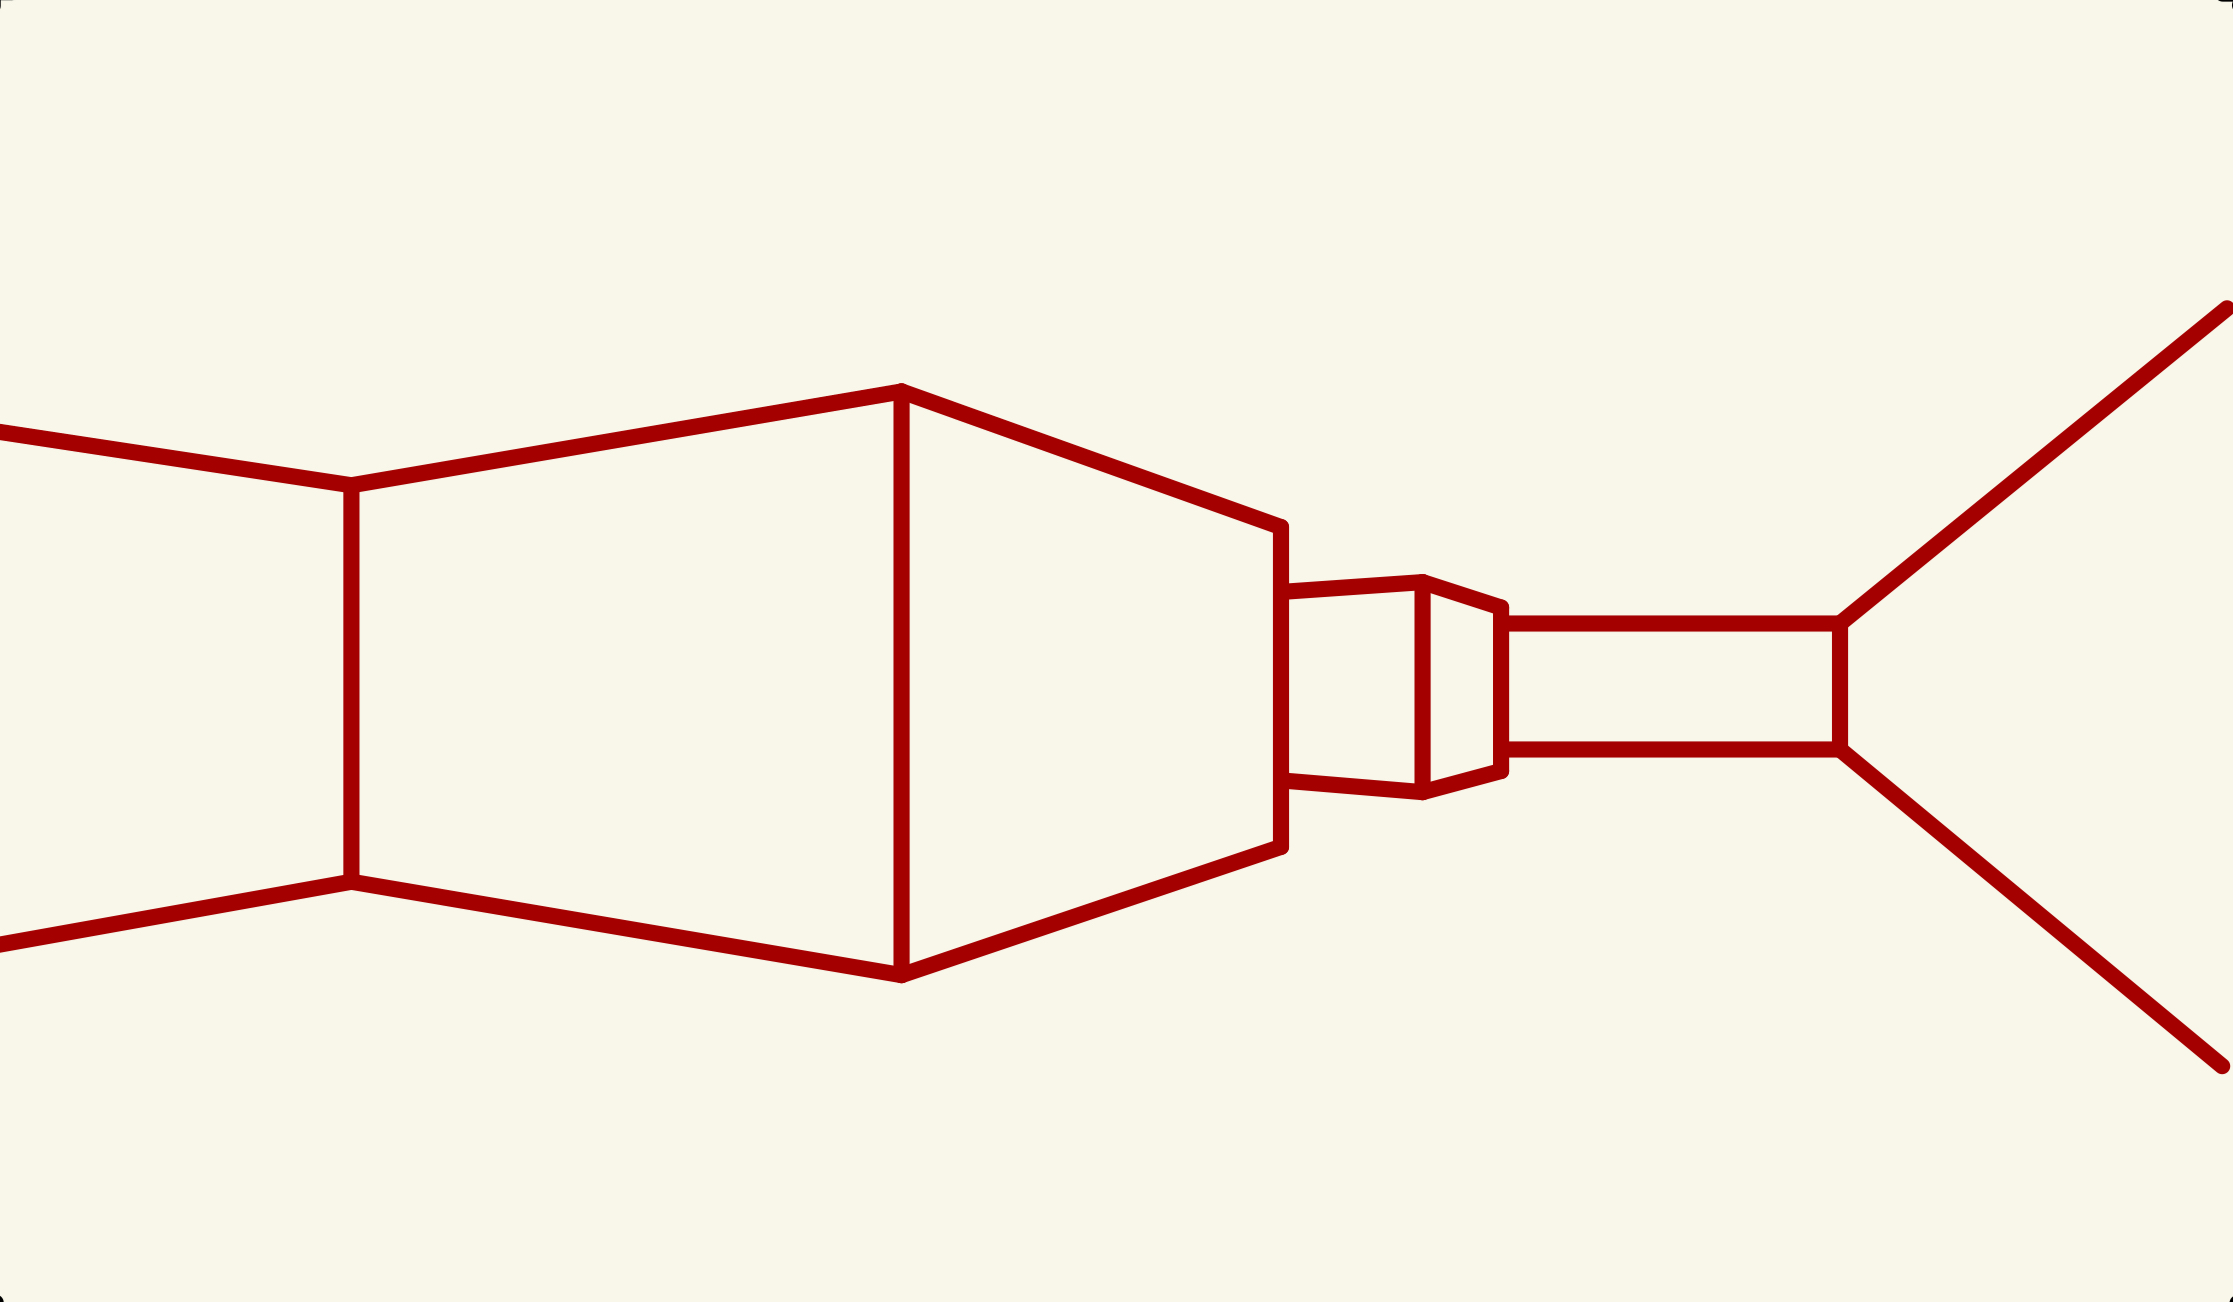
\includegraphics[width=0.6\textwidth]{image/rendu-sans-texture.jpeg}
	\caption{résultat moderne attendu}
	\label{fig:result-modern}
\end{figure}

Cette seconde approche s'approche des algorithme \textit{Line Of Sight} et consiste à calculer la distance entre le 
joueur et chaque sommet de chaque mur.
Pour ce faire, on a pu récupérer l'algorithme DDA précédemment utilisé pour le rendu des murs mais cette fois-ci 
en visant chaque sommet au lieu de viser chaque colonne de pixel. Cela permet théoriquement de réduire considérablement 
le nombre de calculs à effectuer (cf: \nameref{fig:result-modern}).

\paragraph{Cependant, des cas particuliers sont à considérer :}
\begin{itemize}
	\item \textbf{Viser un sommet avec DDA : } Si DDA est efficace et précis cela peut être la cause de certains problèmes. 
	En effet, si l'on vise un sommet de mur avec un rayon, la moindre approximation dans le calcul de l'angle avec lequel on 
	lance le rayon ferait rater le sommet en moyenne une fois sur deux.

	\textbf{Solution : }Pour remédier à cela, nous avons ajusté DDA pour qu'à chaque fois qu'un pas
	passe assez proche d'un sommet, si l'une des quatre cellules adjacentes est
	un mur alors on considère que le rayon a touché le sommet.

	\item \textbf{Continuer le rayon après avoir touché un sommet :} Si l'on touche un sommet avec 
	un rayon, il faut déterminer si le rayon doit continuer ou non. Cela est important dans le cas où l'on 
	est au bord d'un mur est qu'il faut faire le rendu du mur se trouvant derrière.

	\textbf{Solution : }Pour déterminer si le rayon doit continuer ou non, il faut regarder si
	dans les cellules adjacentes au sommet touché, il y a exactement un mur et que ce mur
	ne se trouve pas dans la direction du rayon. Si c'est le cas alors on lance un nouveau rayon 
	partant du sommet touché dans la même direction que le rayon précédent (cf: \nameref{fig:3cas-dda}).

	\item \textbf{Récupérer les sommets touchés dans le bon ordre :} Pour afficher tous les murs correctement,
	nous avons rangé les sommets dans l'ordre croissant de leur angle par rapport au joueur. Cela permet d'afficher
	les murs par segments en prenant les sommets deux par deux. Cependant, dans certains cas, le premier sommet 
	dois être relié au dernier sommet.

	\textbf{Solution : }Pour identifier ces cas, nous regardons si dans la liste des sommets, il y a au moins
	un segment qui en contient un autre. Si c'est le cas alors on lie le premier sommet au dernier.

	\item \textbf{Impossibilité de générer les murs à plus de 180° :} Lorsque l'on a envoyé tous les rayons,
	afin de générer tous les murs visibles par le joueur, si l'on essaie de projeter un mur se trouvant derrière
	le joueur sur le plan de projection, alors la projection se retrouve de l'autre coté du plan en symétrie 
	par rapport au joueur. Concrètement, cela signifie que la carte graphique ne peux pas gérer ces mur les
	affichant alors devant le joueur.

	\textbf{Solution : }Pour régler ce problème, il faut créer une droite imaginaire passant par le 
	joueur et orthogonale à la direction dans laquelle le joueur regarde. Ensuite, il faut retirer
	tous les segments qui se trouvent de l'autre coté de cette droite. Puis, il faut ajouter un sommet
	à l'intersection de cette droite avec chaque segment l'intersectant, en plaçant ces points, 
	légèrement décalé de l'intersection entre la droite et le segment, car sinon il serait impossible de
	projeter ce point sur le plan de projection, le plan étant lui même parallèle à la droite. Enfin, 
	on peut générer les murs comme précédemment.

	\item \textbf{Afficher des textures sur les murs :} Pour afficher des murs texturés, il faut
	pouvoir mapper une texture sur un trapèze en deux dimensions. Cependant il ne suffit pas d'afficher 
	une texture coupé en deux triangles. En effet, il faut que la déformation soit correcte
	du point de vue de la perspective et ce problème est loin d'être trivial.

	\textbf{Solution : }Ce problème étant très complexe à régler, nous avons décider de choisir
	une autre méthode qui consiste à couper le trapèze en six triangles choisis de telle 
	sorte que la déformation ne soit pas trop flagrante. Cela dit, cette méthode empêche 
	l'utilisation de textures avec des motifs réguliers et principalement horizontaux.
\end{itemize}
\begin{figure}
	\center\begin{minipage}{\textwidth}
		\center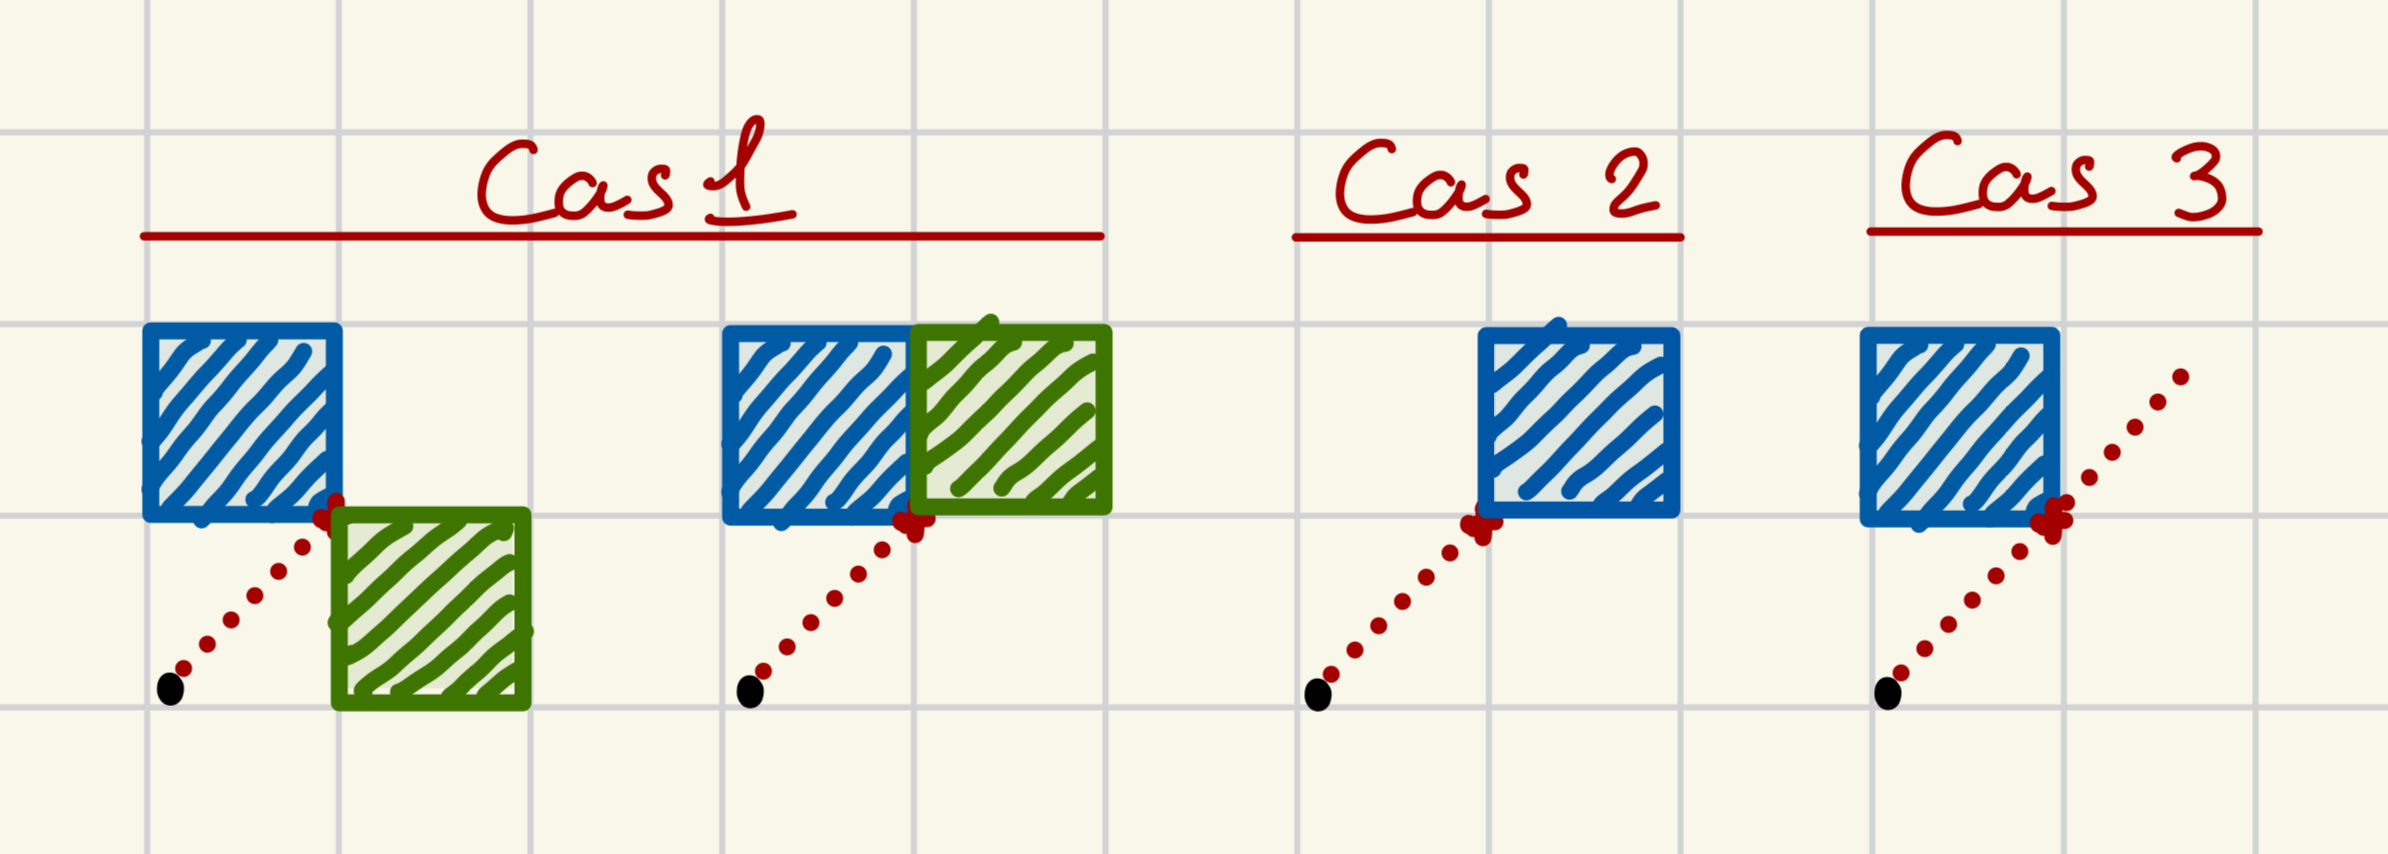
\includegraphics[width=\linewidth]{image/3cas-dda.jpeg}
		\caption{Les 3 cas de projection de rayon à gérer}
		\label{fig:3cas-dda}
	\end{minipage}
\end{figure}




\section{Implantation}

\subsection{La boucle de jeu}
Dans cette partie nous allons détailler les différentes étapes de la boucle de jeu.

\paragraph{Events:}
Nous allons tous d'abord gérer la gestion des évènements. Pour cela nous allons effectuer une boucle sur les évènements et pour chaque bouton sur lesquels nous avons ajouté une action, nous allons effectuer cette action. Nous allons aussi gérer les fonctions de déplacement de la vision grâce à la souris avec la position relative de la souris. Ensuite, nous allons gérer la fonction d'envoie des portails en fonction du clic de la souris effectuer.

\paragraph{Update:}
Nous allons effectuer une update du jeu par rapport au temps écoulé depuis le dernier update. Cette update va permettre de mettre à jour (les attributs du joueur). De calculer la nouvelle position du joueur si il est en colision avec un mur. Et enfin calculer les nouveaux attributs du joueur si il est proche d'un portail lorsque les deux portails sont activés.

\paragraph{Render:}
Avant de faire le nouveau rendu des entités, nous allons d'abord effacer tous les rendus précédents. Ensuite nous allons effectuer le rendu de toutes les entités que nous allons détaillés dans la parties suivante.



\subsection{Le rendu des murs:}

\begin{figure}
	\begin{minipage}{\textwidth}
		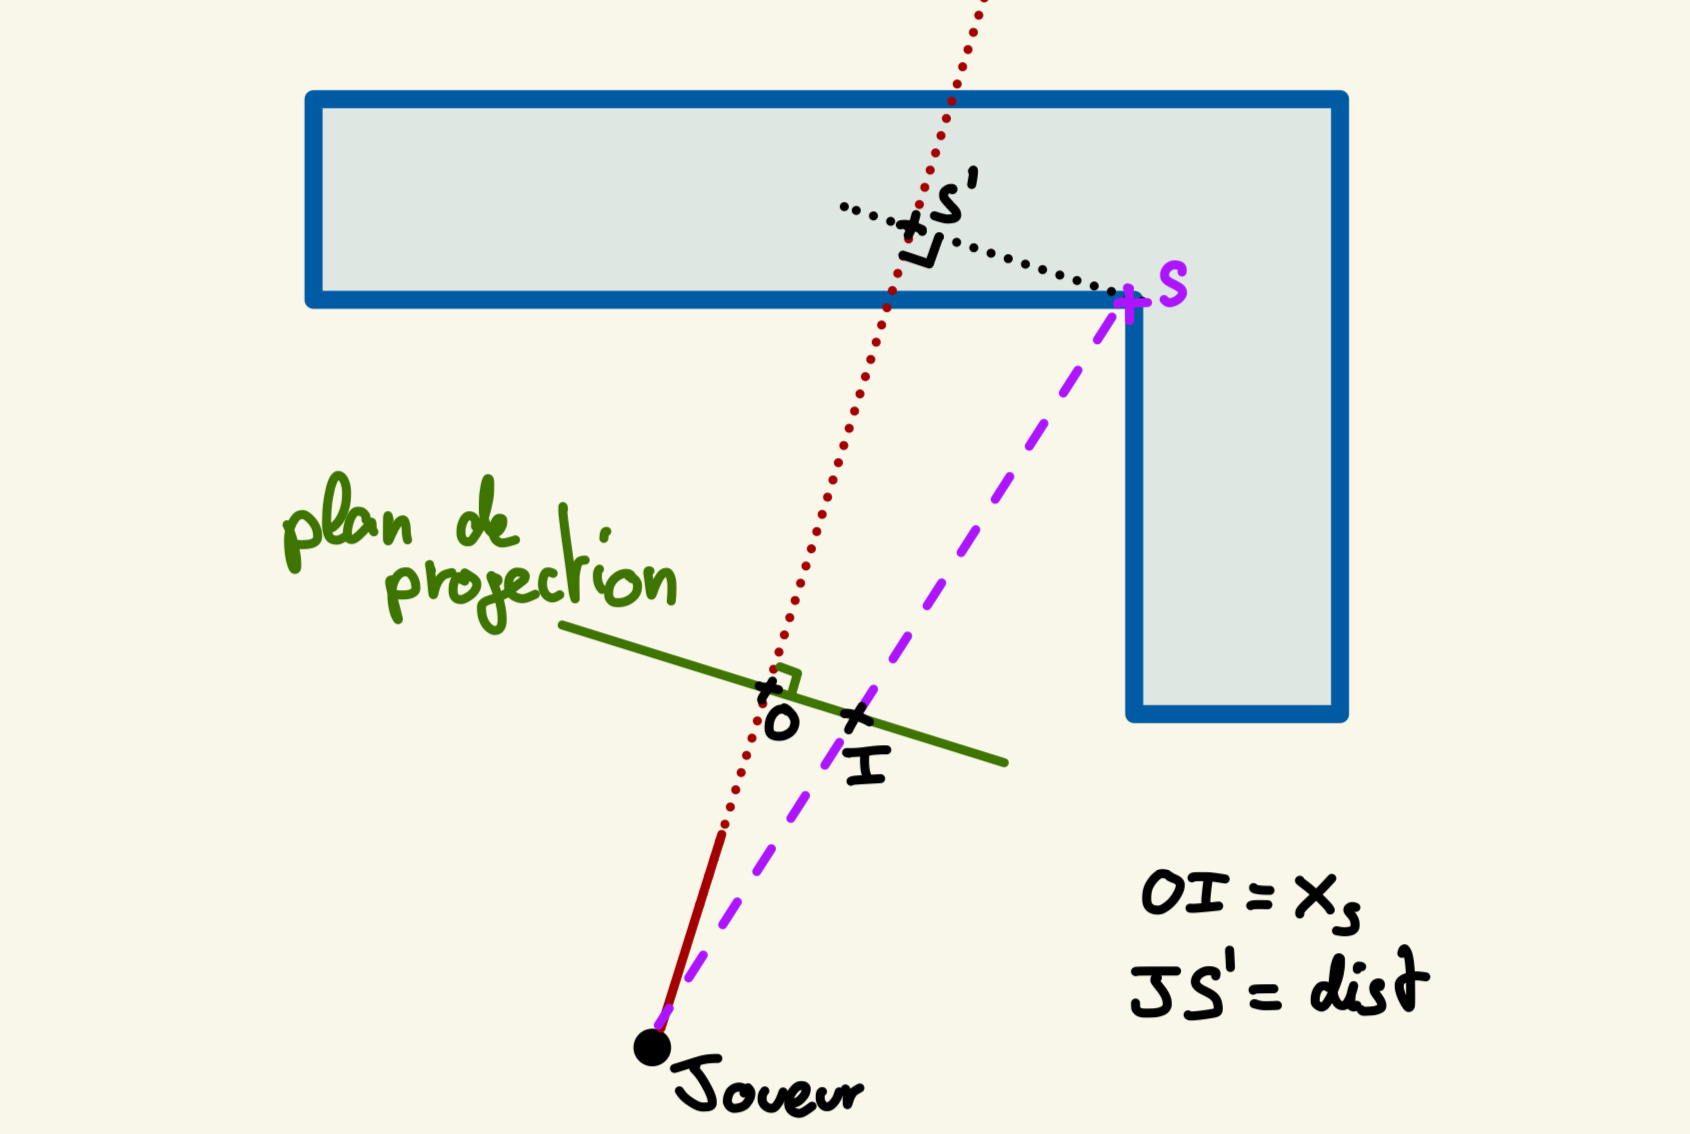
\includegraphics[width=\linewidth]{image/shemaLanceRayon01.jpeg}
		\hspace*{-0.5cm}
		\caption{Lancé d'un rayon}
		\label{fig:shemaLanceRayon01}
	\end{minipage}
\end{figure}


Pour le rendu des murs, tous les sommets de chaque mur sont récupérés et triés selon leur angle par rapport au joueur.
Ensuite, ces sommets sont parcourus dans ce nouvel ordre pour y envoyer un rayon grâce à DDA. Connaissant alors l'angle
avec lequel le rayon est envoyé, la distance entre le joueur et le sommet est calculée en prenant le projeter orthogonale
du sommet sur la droite de direction de vue du joueur (cf : \nameref{fig:shemaLanceRayon01}). Avec ces deux informations, nous pouvons alors calculer le projeté
du sommet sur le plan de projection. Chaque sommet de mur est, sur la carte en 2D, un point. Sur le plan de projection, 
ces sommets sont représentés par un segment vertical. Il faut donc, pour projeter un sommet sur le plan de projection, connaître
deux points. Ces points étant verticalement alignés, il faut déterminer l'abscisse commun à ces deux points et leur ordonnée 
respectives. Les deux points étant une symétrie l'un de l'autre par rapport à la droite horizontale passant par le centre du plan,
il nous faut connaître deux informations seulement : l'abscisse du sommet sur le plan et la distance entre le joueur et le sommet
afin d'en déduire la taille du sommet (cf: \nameref{fig:shemaLanceRayon01}) : \\

On pose $(x_j, y_j)$ les coordonnées du joueur,  $(x_s, y_s)$ celles du sommet, $W$ la largeur de la
vue et $H$ sa hauteur. On a alors : \\
\begin{itemize}
	\item[] \textbf{Pour l'angle du sommet : } \\
	\[
		\theta = atan2(y_s - y_j, x_s - x_j)
	\]

	la fonction $atan2(y, x)$ permet de calculer l'angle entre l'origine du plan et le point (x, y).

	\item[] \textbf{Pour la distance du sommet : } \\
	\[
		dist = \cos(\theta - \theta_{joueur})\sqrt{(x_s - x_j)(x_s - x_j) + (y_s - y_j)(y_s - y_j)}
	\]
	
	\item[] \textbf{Pour l'abscisse des deux points : } \\
	\[
		x = \frac{W\tan(\theta -  \theta_{joueur})}{2}
	\]

	\item[] \textbf{Pour la hauteur du segment vertical : } \\ 
	\[
		h = 
		\begin{cases}
			\frac{H}{2dist} & \text{si } dist \neq 0 \\
			2H & \text{sinon }
		\end{cases}
	\]
\end{itemize}

On obtient alors les deux points du segment représentant le sommet sur le plan comme suit :
\begin{align*}
    P_1 &= (x + \frac{W}{2}, \frac{H}{2} - \frac{h}{2}) \\
	P_2 &= (x + \frac{W}{2}, \frac{H}{2} + \frac{h}{2})
\end{align*}


\subsection{Les portails}

Le personnage dispose d’un portail bleu et un portail orange que l’on activent en utilisant le clique droit et gauche.
Ils se positionnent chacun sur un mur.
Les portails servent à créer un passage d’un point A à un point B pour ainsi gagner de la distance et du temps.

Pour utiliser les portails, il faut commencer par poser les deux portails.
Ensuite, il faut se déplacer en continue contre l’un des deux portails ce qui permet de sortir par l’autre.

D’un point de vue technique, nous utilisons une structure qui contient :

\begin{align*}
    \text{(float;float) coords} & \xrightarrow{} \text{Les coordonnées du portail} \\
    \text{int dir, dir } \in \mathopen{[}0\,;3\mathclose{]} & \xrightarrow{} \text{La direction du portail} \\
    \text{portal* other} & \xrightarrow{} \text{Un pointeur sur le portail associé} \\
    \text{int width} & \xrightarrow{} \text{La largeur du portail}
\end{align*}

Pour positionner un portail lors d’un clique, on récupère le point d’inter\-section entre la direction regardée par le personnage et le premier mur rencontré. 
Ce point sert alors de coordonnées à notre portail. 

Pour connaître la direction\footnote{Si le portail est sur la droite, la gauche, le haut ou le bas d’un mur} du portail, nous voyons d’abord si le mur utilisé comme support est vertical ou horizontal. 
Si le mur est vertical (resp. horizontal) alors si l’abscisse (resp. ordonnée) du personnage est inférieur à l’abscisse (resp. ordonnée) du mur, alors le portail est posé sur la gauche (resp. le haut) du mur. Sinon  le portail est posé sur la droite (resp. le bas) du mur.

Pour savoir si le personnage rencontre un portail, on utilise le même système de collision utilisé avec les murs et l’on vérifie les collisions avec les portails avant celles des murs.

Pour effectuer le passage d’un portail à l’autre, on doit calculer les nouvelles coordonnées du personnage (noté C) ainsi que l’angle (noté $\alpha$) indiquant sa direction. Les portails sont notés Pe (portail d’entrée) et Ps (portail de sortie).
En ce qui concerne le nouvelle angle, on utilise la direction des portails et l’angle actuel du personnage (noté $\beta$). La relation suivante permet de calculer cet angle :

$$\alpha = \beta + \pi + (\text{Ps.dir} – \text{Pe.dir}) \times \pi / 2$$

Cette relation utilise la différence entre les directions des portails pour connaître le nombre de quart de tour nécessaires. On doit ajouter un demi-tour et l’angle actuel du personnage pour garder l’orientation du personnage.

Pour trouver les nouvelles coordonnées, on réutilise les directions des portails. On effectue une superposition imaginaire entre les portails et l’on doit transformer les coordonnées pour avoir une suite logique à travers les portails.

Il y a quatre possibilités de nouvelles coordonnées et chacun des cas correspond au résultat du calcul suivant :

$$\text{Ps.dir} + \text{Pe.dir} \equiv n (4)$$

\begin{center}
    \begin{tabular}{c|l}
            $n$ & nouvelle position associée \\
            \hline
            0 & $(\text{Ps}.x + (\text{J}.x - \text{Pe}.x) ; \text{Ps}.y - (\text{J}.y - \text{Pe}.y))$ \\ 
            1 & $(\text{Ps}.x + (\text{J}.y - \text{Pe}.y) ; \text{Ps}.y + (\text{J}.x - \text{Pe}.x))$ \\
            2 & $(\text{Ps}.x - (\text{J}.x - \text{Pe}.x) ; \text{Ps}.y + (\text{J}.y - \text{Pe}.y))$ \\
            3 & $(\text{Ps}.x - (\text{J}.y - \text{Pe}.y) ; \text{Ps}.y - (\text{J}.x - \text{Pe}.x))$ \\
    \end{tabular}
\end{center}

Notations :

- Pe.$x$ (resp. Pe.$y$) → abscisse (resp. ordonnée) du portail d’entrée

- Ps.$x$ (resp. Ps.$y$) → abscisse (resp. ordonnée) du portail de sortie

- J.$x$ (resp. J.$y$) → abscisse (resp. ordonnée) du joueur/personnage

Nous avons donc les nouvelles coordonnées ainsi que le nouvel angle du personnage.

\section{Conclusion}
\subsection{Bilan technique}
\subsection{Améliorations possibles}
\subsubsection{Améliorations de l'existant}

\begin{figure}
	\begin{minipage}{\textwidth}
		\center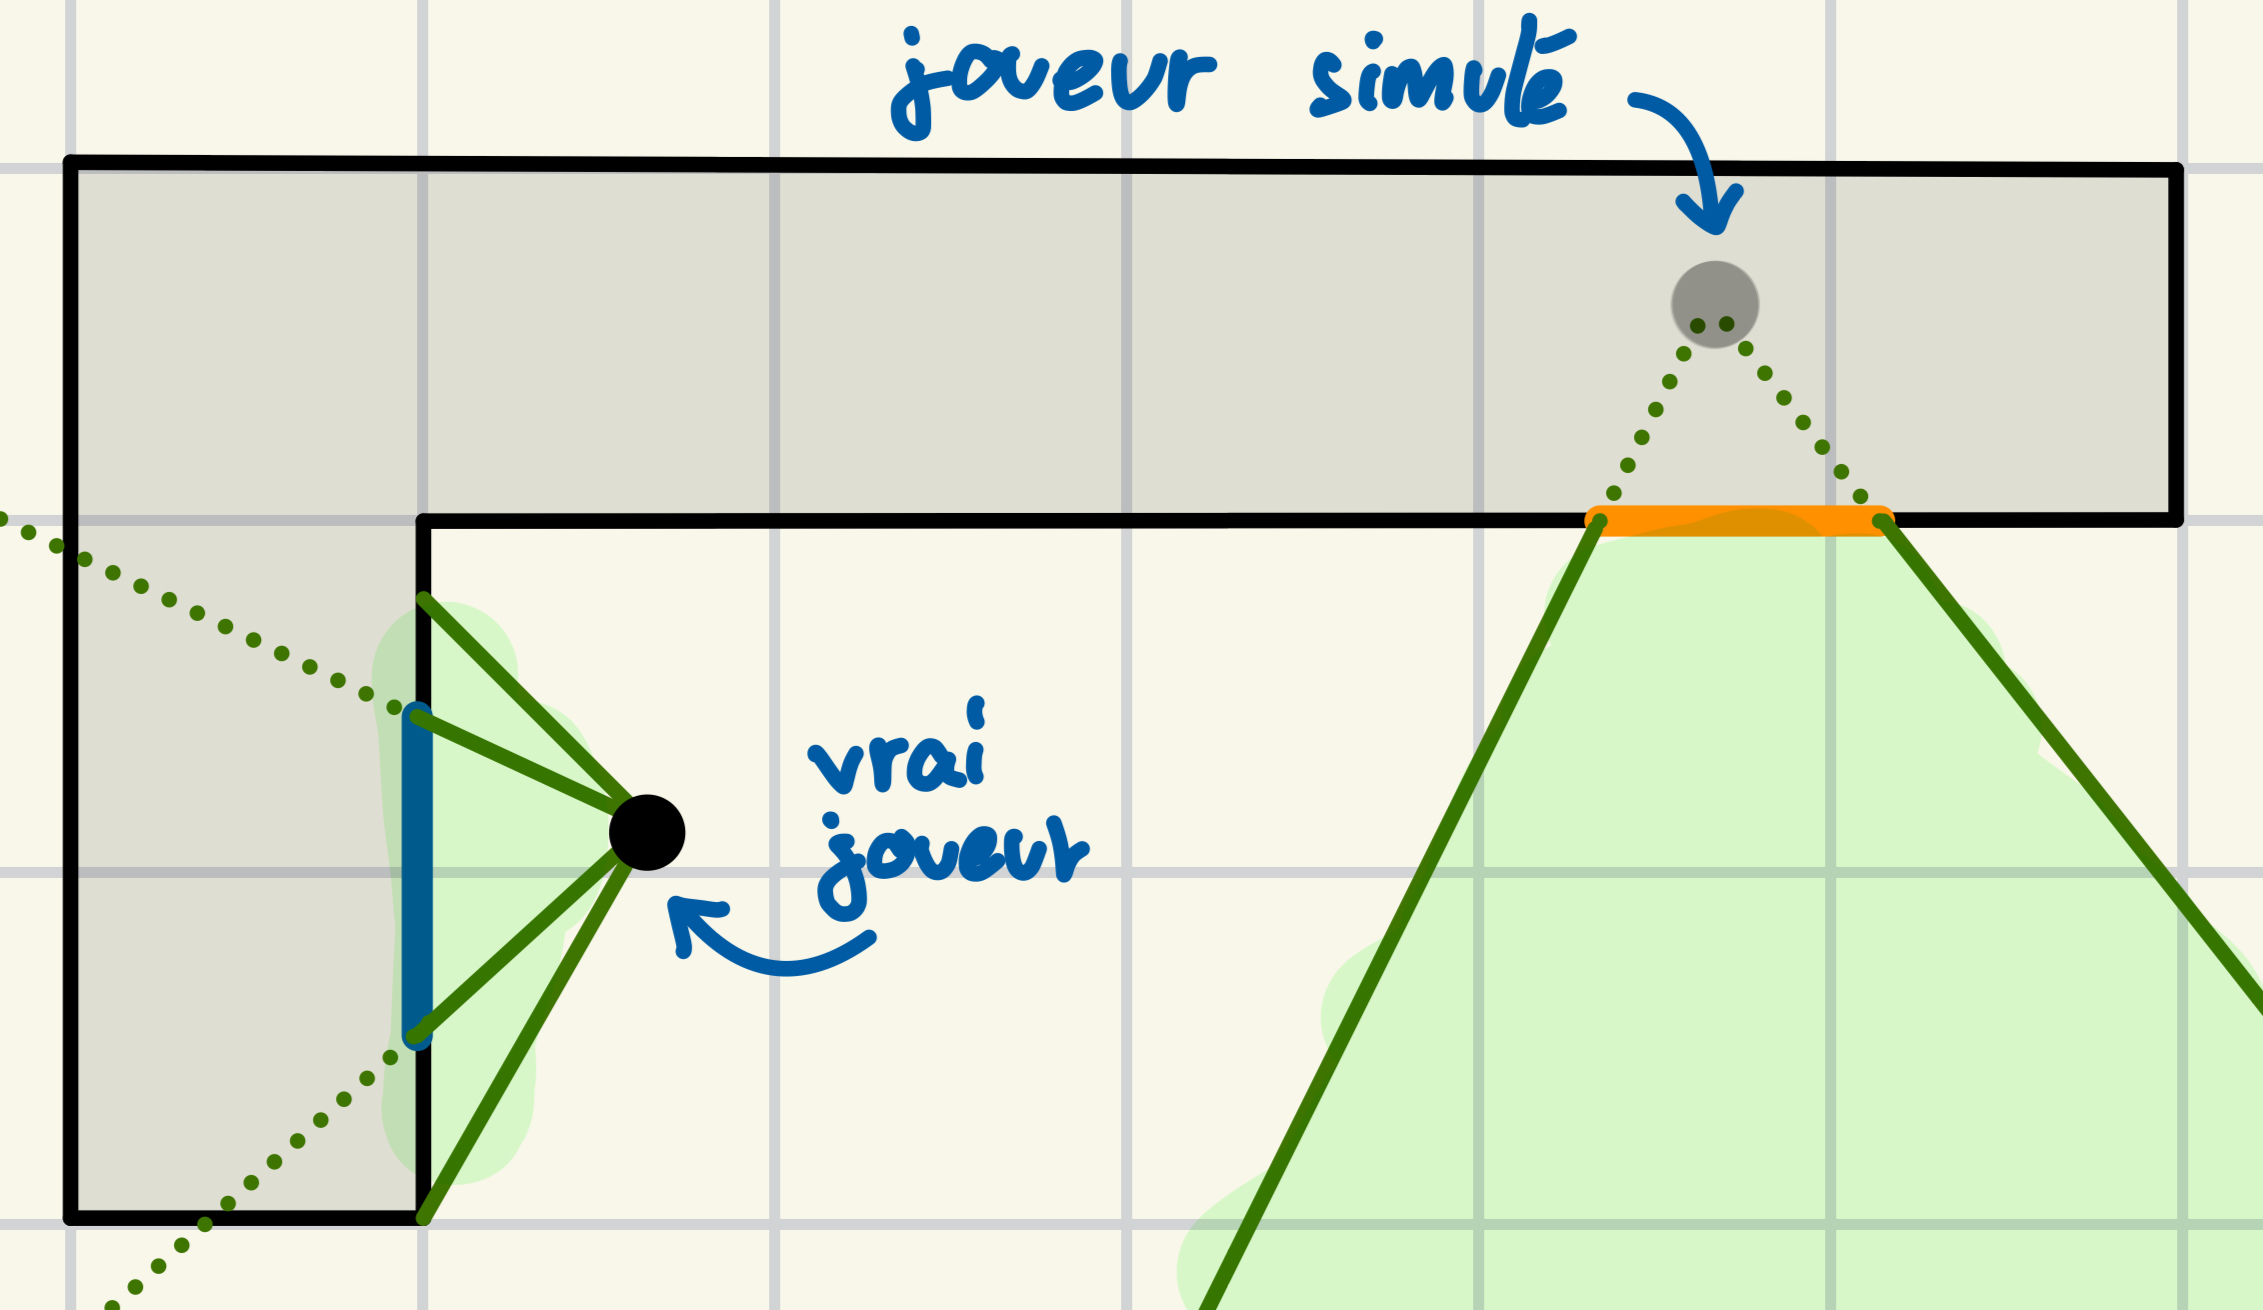
\includegraphics[width=0.8\linewidth]{image/vue-travers-portail.jpeg}
		\hspace*{-0.5cm}
		\caption{Vue à travers un portail}
		\label{fig:vue-travers-portail}
	\end{minipage}
\end{figure}

La plus grande amélioration possible serait de pouvoir voir à travers les portails
lorsque les deux sont activés.

Pour cela, on pourrais simuler un joueur se trouvant derrière le portail
lié à celui au travers duquel on regarde. On pourrais alors afficher
ce que ce joueur simulé voit à travers le portail (cf: \nameref{fig:vue-travers-portail}). 

Il faudrait cependant alors créer un nouveau type de rendu car le joueur
simulé étant derrière le portail lié, il se trouverais derrière ou à l'intérieur
d'un mur. On pourrais alors imaginer une façon de ne pas prendre en compte tous ce qui 
se trouve derrière le portail d'un point de vue affichage mais aussi 
d'un point de vue du lancé des rayon aui ne doivent pas s'arrêter sur
un mur derrière le portail lié.

\subsubsection{Nouvelles fonctionnalités}

Parmi de nouvelles fonctionnalités, que nous pourrions rajouter en voici quelques unes:
\begin{itemize}
	\item Permettre à l'utilisateur de créer ses propres cartes
	\item Avoir des murs où il est impossible de tirer un portail
	\item Avoir des endroits au sol que lorsqu'on marche dessus, on est téléporter à la case départ
	\item Pouvoir mettre plusieurs textures différentes sur les murs
	\item Avoir des murs qui possèdent des trous permettant de voir ainsi que tirer des portails à travers
\end{itemize}

\newpage

% \section{Bibliographie}
\bibliographystyle{plain}
\bibliography{references}


\newpage
% 4ème de couverture
\thispagestyle{empty}
\section*{Résumé}
Ce rapport présente le projet Portal 0.0, un préquel au jeu portal de Valve.
Portal 0.0 utilise un moteur 3D appelé Raycaster, un moteur très populaire
dans les années 90, popularisé par des jeux comme Wolfenstein 3D.

Les objectifs de ce projet étaient de créer un jeu en 3D  en C++ avec la bibliothèque
Gamedev Framework (GF), en utilisant le raycasting
et de permettre au joueur de se déplacer dans un environnement en 3D, de tirer des portails,
de les traverser et de voir au travers.

Ce projet à résulté en un jeu fonctionnel avec des murs en 3D 
affiché par raycasting. Le joueur peut se déplacer dans l'environnement,
tirer des portails et les traverser. 

Des améliorations sont cependant possibles. Il pourrais être intéressant
de finalement permettre au joueur de voir à travers les portails 
lorsqu'ils sont activés. Aussi, il serait intéressant de permettre
à l'utilisateur de créer ses propres cartes.

\paragraph{\textbf{Mots clés :}} Raycasting, 3D, C++, Gamedev Framework, Portails, Jeu vidéo.

\hrulefill

\section*{Abstract}
This report presents the Portal 0.0 project, a prequel to Valve's Portal game. Portal 0.0 utilizes a 3D engine called Raycaster, a very popular engine in the 90s, popularized by games like Wolfenstein 3D.

The objectives of this project were to create a 3D game in C++ using the Gamedev Framework (GF), utilizing raycasting to allow the player to navigate a 3D environment, shoot portals, traverse them, and see through them.

This project resulted in a functional game with 3D walls displayed through raycasting. The player can move around the environment, shoot portals, and traverse them.

However, there are potential improvements. It could be interesting to finally allow the player to see through the portals when they are activated. Also, it would be interesting to allow the user to create their own maps.

\paragraph{\textbf{Keywords :}} Raycasting, 3D, C++, Gamedev Framework, Portals, Video Game.

\end{document}
